\chapter{Usability Study}
\label{USABILITY_STUDY}

  The aim of this usability study is to compare the usability of three popular distributed computing systems: Apache Hadoop MapReduce; Apache Spark; and Apache Flink, thus providing data for the usability component of the systems' multidimentional comparison. The participants of this usability study were masters students from a cloud computing class at the University of Sydney, where the mentioned systems were taught. The focus of that course is on data processing in the cloud, assessed with practical programming assignments. Stream processing is not covered in this course or the usability study -- all exercises are in the form of batch processing.
  
  As highlighted in the related work section, our study is quite novel and unique as the two closest existing usability studies of similar circumstance still differed fundamentally in scope and study duration. We adapted effective study design considerations from those and other papers where possible, and otherwise applied our knowledge and best judgment in designing this usability study. This section will describe the background of the study, the study design and decisions that were made in its regard, and the strengths and challenges in its execution.


\section{Background}

  The usability study was conducted as part of a regular master's level class on cloud computing at the University of Sydney. This class attracts a diverse student cohort because it is available for selection in several different degrees, most prominently including students studying computer science at either master's or undergraduate (4th year) level, or studying a Master of Data Science -- which does not require a computer science background. Participation in this study was voluntary, so it was paramount to design and organise the usability study in such a way that students who did not opt-in to participate were not at an advantage or disadvantage. 

  The class of 2017 was scheduled to start in early March, and consideration and preparation for this usability study began in early-mid February. Topics relevant to the usability study began being taught in early April through to late June, with the earlier weeks dedicated to general concepts like the cloud and data centres. Thus the time-frame for the usability study was 2.5 months, with 1.5 months preparation.

  The author of this thesis and his supervisor both held roles in execution of the unit of study while the study was being performed. A. Prof. Uwe R\"ohm was the unit of study coordinator and lecturer. Bilal Akil was the unit of study teaching assistant and one of its five tutors. Thus, once granted ethics approval, we had the means to reshape the class to better fit the usability study -- bearing in mind the students who may not have opted-in.

  In previous years, this course covered Apache Hadoop MapReduce and Apache Spark, and this year a third system -- Apache Flink -- was taught too. A YARN enabled cluster was available to this course's students, and needed Apache Flink installed and all relevant systems updated. Teaching material and exercises were prepared for all three systems and updated where necessary. Because of the diversity of the student cohort, this course supports both the Java and Python programming languages, which individual students can select as they prefer. This means six variants of exercise and assignment solutions (3 systems $\times$ 2 programming languages) were prepared.

  We realised that the preparation time was not long enough to address everything before the usability study commenced. Assignments and learning materials would need to be developed and the cluster would need to be updated as the usability study was being executed. With this in mind, time being a scarce resource was a factor that had to be considered in the study's design.

  The assessment component of the class comprised three practical programming assignments that students worked on in pairs, plus a written final exam that is not part of this study. Students were provided with between three and four weeks to complete assignments, each of which were an increasingly complex series of distributed computing tasks in some domain.


\section{Design}

  To be fair to all the class' students, we decided that they would all learn and use each of the three distributed computing engines, as opposed to dividing usage among them. This choice was made to avoid circumstances such as: ``Why did (s)he use System X but I had to use System Y?''
  
  Each assignment was targeted at different distributed computing engines (cf. Table~\ref{TABLE:ASSIGNMENTS_OVERVIEW}), and provided students with an experience which they could then reflect upon to consider the usability of each system. The first assignment covered the lower level framework, Apache Hadoop MapReduce. This placed participants on an equal starting point for comparison to the more modern, higher level data processing frameworks to come. This decision also complemented the existing course structure, where the fundamental and lower level distributed computing concepts are taught first. We suspected that the majority of participants would \emph{not} prefer to use Hadoop MapReduce compared to the other systems (and you can see in Section~\ref{ANALYSIS} that this was indeed the case), and thus were not concerned by the possibility of slight biases in favour of it that may be introduced by having used it first.

  On the other hand, we were concerned that the order of usage for the next two systems could have an effect on their comparison results -- or at least that it would be difficult to be confident that they would not. To account for this, we decided to employ a crossed A/B test for the remaining two assignments: half of the participants used Apache Spark for assignment 2 and Apache Flink for assignment 3, and the other half did the opposite. Therefore teaching and learning resources for both systems were to be made available at the roughly same time and depth.


\subsection{Assignment Tasks}

  \begin{table}[ht]
    \scriptsize
    \centering
    \setlength\tabcolsep{3pt}
    
    \caption{Overview on programming tasks used in study.}
    \label{TABLE:ASSIGNMENTS_OVERVIEW}

    \makebox[\textwidth]{\begin{tabular}{l | c c l l}
      \toprule
                            & \textbf{System}     & \textbf{Scenario} & \textbf{Data set}               & \textbf{Tasks}                                                                \\
      \midrule
      \textbf{Assignment 1} & Hadoop MR           & Social media      & Flickr: Photos, locations, tags & \textbf{Basics} (filter, transpose, join, aggregation), ranking               \\
      \textbf{Assignment 2} & Flink $\vert$ Spark & Immunology        & Cytometry $+$ experiment data   & \textbf{Basics}, iteration: $k$-means clustering \cite{hartigan1979algorithm} \\
      \textbf{Assignment 3} & Flink $\vert$ Spark & Genomics          & DNA microarray $+$ patient data & \textbf{Basics}, iteration: Apriori algorithm \cite{agrawal1994fast}          \\
      \bottomrule
    \end{tabular}}
  \end{table}

  An overview of the assignment scenarios and tasks that were used in the usability study can be seen in Table~\ref{TABLE:ASSIGNMENTS_OVERVIEW}. The main design considerations for the practical assignments were:

  \begin{itemize}
    \item The change from two systems and assignments in the past to three was expected to increase the difficulty of the course. Considering this, the assignments were made smaller, requiring about two weeks for a pair to complete instead of three or four.
    \item Each assignment used a different data set to avoid having participants become accustomed to the same one.
    \item All data sets had schemas of similar complexity -- two to three tables given as CSV files that could be joined on a foreign key relationship, and one list-valued attribute that had to be transposed during querying.
    \item The first assignment required participants to exercise various distributed computing operations: map, reduce, filter, group and ranking. Being in Apache Hadoop MapReduce, the latter 3 required non-trivial implementation.
    \item The second and third assignments also covered declarative analysis with filtering, join and aggregation to allow comparison back with Hadoop MapReduce.
    \item Additionally, the last two assignments involved a task focused around some iterative data mining algorithm.
  \end{itemize}
  
  It was recognised that the difficulty of each assignment was variable, considering the changing systems (particularly from the lower level MapReduce in assignment 1 to the higher level systems), scenarios, data sets, and algorithms. However, these were all necessary either for the reduction of bias towards any particular system, or for the general flow of the course. Effects that assignment difficulty may have had on perceived usability has been explored in Section~\ref{ANALYSIS}.

  We intended to include assignment marks in the usability study data. Since the unit of study had multiple tutors to teach classes and mark assignments, it was necessary (more than otherwise) to implement some form of marking that would reduce subjectivity and thus potential bias from individual markers. We tried taking on the approach described in section 6.4 of the study by \citeauthor{NANZ:CONCURRENCY_STUDY:2013} \cite{NANZ:CONCURRENCY_STUDY:2013}: to identify a set of mistakes and their weightings, and then to perform marking backwards, so to speak. However we faced a challenge when trying to implement this, wherein our course structure required the release of a marking rubric for students to access prior to completion of the assignment, inferring that the set of potential mistakes had to be compiled beforehand, as opposed to after scanning submissions and categorising the mistakes that actually were made -- as performed in the reference paper. Ultimately it was decided to exclude assignment marks from the study.


\subsection{Data Analysis Scenarios}

  Each assignment was set in a different scenario to avoid any potential bias due to familiarity with a data set (cf. Table~\ref{TABLE:ASSIGNMENTS_OVERVIEW}). As our aim is to study the usability of the distributed data processing platforms for non-computer scientists (those who would have difficulty judging usability and such on their own), we chose data analysis scenarios from social media, bioinformatics, and genomics.
  
  Assignment~1 involved data analysis of Flickr data. The data set is an excerpt of real-world Flickr data including a hierarchical location attribute and multiple tags per photo given as a multivalued attribute. Students were asked to implement different analytical queries to identify: the number of photos taken at a certain locality level; the top 50 localities by number of photos; and the top 10 tags used for those photos.
  
  Assignment~2 considered a scenario from immunology, involving real cytometry data from a study of infections with the West Nile Virus. We also attached fabricated metadata to the real cytometry data, for instance information about the imaginary researcher who collected the data, to facilitate examination of particular skills. This assignment had two subtasks. Firstly, students had to determine the number of valid measurements per researcher, involving: filter; transpose; join; and aggregation operations, similar to assignment~1. Secondly, students had to complete a clustering task to identify similar cell measurements with regard to some given 3-dimensional cell markers using the $k$-means clustering algorithm \cite{hartigan1979algorithm}.
  
  Assignment~3 presents a genomics scenario requiring the analysis of a DNA microarray data set and patient metadata. This data set was synthetic -- generated using the schema and data generator from the GenBase benchmark \cite{TaftVSSMS:SIGMOD2014}. We modified the GenBase schema to allow the application of multiple disease codes per patient (instead of a single one) via a multivalued attribute. Students were first asked to find the number of cancer patients with certain active genes, covering the filter, transpose, join, and aggregation operations as in the previous two assignments. They further had to mine the microarray data in search of frequent combinations of expressed genes for certain cancer types using the Apriori algorithm \cite{agrawal1994fast}.


\subsection{Self-Reflection Surveys}

  We included a short survey as part of the assignment submission process, acting as a method of self-reflection for students after completing the assignment, and also as a primary source of the usability study's data. The survey was only available for completion following the submission of source code, thus capturing their view of each system upon completion of the relevant assignment, as opposed to say halfway through.

  Although the assignments were completed in pairs, and thus only one source code submission was necessary for a pair of students, we emphasized that the self-reflection surveys were to be completed individually.

  The surveys for each assignment included:

  \begin{itemize}
    \item A simple and standard usability survey: the System Usability Scale survey \cite{BROOKE:SUS:1996}, as discussed in Section~\ref{SUS}.
    \item A question directly asking which is their preferred system. This question does not apply to assignment 1.
    \item A question asking approximately how much time was spent working on the assignment. Options were separated into seven 4 hour bins, from 0-4 hours, to 20-24 hours and then 24+ hours.
    \item A text area to provide any textual feedback.
  \end{itemize}
  
  The first survey also included four questions to gauge students' prior programming experience. It asked how many years of programming experience the students considered themselves to have, from 0 to 9 and then 10+, and three Likert scale questions asking students for their perceived proficiency with Java, Python and shell environments, from ``No proficiency'' to ``Very high proficiency''.
  
  We required all students to complete the survey as part of their learning outcomes, as we considered it a form of self-reflection. However, all questions were optional, allowing students to omit any if uncomfortable. Only participating students' survey data was included for the purpose of the usability study. We made sure to keep the survey brief and simple to reduce load on students and, perhaps optimistically, reduce fake responses and increase usability study participation.


\subsection{System Usability Scale (SUS)}
\label{SUS}

  The SUS \cite{BROOKE:SUS:1996} was used to provide a score for the usability of each system to be used for comparison. While programming frameworks or distributed systems may not be the intended application of this survey, we were unable to find anything more specifically targeted to this use case, and found that the SUS was general enough to be applied nonetheless, considering that our survey was explicitly focused on usability. In this regard we were trying something seemingly rare, and thus could not be sure of the applicability of the results.
  
  The SUS is comprised of ten Likert scale questions. Odd numbered questions are positively natured, while even numbered are negative. The final score is compiled adding or subtracting those scores and applying a multiplier, becoming a single score between 0 and 100. Note that SUS scores are interval level -- not ratio -- meaning a SUS score of 80 is not necessarily twice as good as 40.
  
  We decided to use this survey as it presented a good balance of ease and generality. Ease here refers to the survey only having ten questions of a simple nature. Generality is in how the survey only presents rather general statements about the `system', making it applicable to a variety of systems even with significant differences between them, and avoiding references which would not apply or would be confusing in a programming context, such as `scenario' in the After Scenario Questionnaire (ASQ) \cite{LEWIS:QUESTIONNAIRES:1995}, or `information' and `interface' in the Computer System Usability Questionnaire (CSUQ) \cite{LEWIS:QUESTIONNAIRES:1995}.
  
  Despite the availability of more succinct questionnaires, we found the SUS to be of a good balance. While not requiring much time or effort to be conducted overall, its questions may have the potential to provide additional information about the systems that could be used to make recommendations. For instance, ``I needed to learn a lot of things before I could get going with this system'' and ``I thought there was too much inconsistency in this system'' both provide insight into specific strengths or weaknesses of the system in question.
  
  The SUS is also a well-established, widely used and scrutinised method. An empirical study of the SUS used nearly 10 years of data to conclude that the survey does effectively fulfil its purpose of attaining a user's subjective rating of a product's usability \cite{BANGOR:SUS_EVALUATION:2008}.
  
  A study of SUS usage with non-native English speaking participants recommended adjusting a single question to reduce confusion \cite{FINSTAD:SUS:2006}, namely changing the 8th statement from `I found the system very cumbersome to use' to `I found the system very cumbersome/awkward to use', and we chose to adopt this for our usability study. Finally, we modified the fourth question by changing `technical person' to `tutor/technical person', hopefully reducing potential confusion as the context in this usability study does not have an obvious definition of who a technical person is.


\section{Execution}
\label{EXECUTION}

  By designing the usability study with the course and students' learning outcomes as the top priority, we were able to frame the usability study as an application of existing data for the purposes of attaining ethics approval. Specifically, the self-reflection survey was to be performed regardless of the usability study, as a part of the students' learning outcomes. Additionally, the crossed A/B test was to be performed as a way for the course to compare students' feedback on Apache Spark and Apache Flink, to determine which systems are most appropriate for usage in future semesters -- again irrespective of this usability study.

  Thus the data was already being collected for the course itself. For the purpose of this usability study, we were to attain ethics approval to use that existing data in performing this analysis and for disseminating any publications. This approach was very effective considering the time limitations in place, and served the needs of the students, the university, and our research, as we were able to implement most changes to the course structure without having to wait for ethics approval. By the time the first self-reflection survey was executed, which included the option to opt-in to this usability study, we had successfully attained ethics approval.

  Students of the cloud computing class had access to a dedicated teaching cluster of 30 nodes for developing and testing their solutions. This cluster was shared among all students and had all systems installed using the same HDFS file system and YARN resource manager. The distributed computing engine versions used were: Apache Hadoop MapReduce v2.7.2; Apache Spark v2.1.1; Apache Flink v1.2.1. Configuration changes from default settings were kept to a minimum. During the installation and testing process, where we tried to ensure that the systems would work from a the perspective of a logged-in student, we experienced cluster multitenancy issues and found little documentation to assist, ultimately requiring a large amount of our time to work around.
  
  We aimed to support both Java and Python as implementation languages, and consequently lecture and tutorial materials were provided in both languages. However, despite our best efforts, we did not succeed in creating exercise materials for Flink with Python that worked well enough that we could instruct students on. We found that some simple operations were behaving unpredictably or producing overly complicated and computationally expensive dataflows, making it very difficult to solve even basic tasks efficiently. There was limited documentation on the matter and the whole experience felt rather immature. Ultimately we did not provide teaching materials for Flink in Python, and recommended that students avoid using it for their assignments. This recommendation was followed as all Flink submissions were written in Java. An exploration of the potential biases this may have introduced was performed in Section~\ref{LANGUAGE_INFLUENCE}.
  
  Due to the delays caused by this struggle, we were forced to release Flink tutorial exercises (only in Java) one week after Spark's, as opposed to the desired synchronised release. This remained prior to release of assignment~2, and lectures still covered both systems in parallel.
  
  We designed the usability study such that the comparisons of Flink and Spark were done in a crossed A/B test to avoid potential bias for or against the first system used after MapReduce. To this end, student pairs were randomly assigned to use Spark or Flink for assignment~2, with an even split.
  
  However, some students requested to change their assigned system for assignment~2 from Flink to Spark. We suspect that this was due to Flink's tutorial exercises having been delayed while working on Python support, meaning students had less experience with it than Spark when assignment~2 was to come around. We did not deny their requests, and instead offered other Spark groups to transfer to Flink in an effort to restore balance. Ultimately there were more students using Spark than Flink for assignment~2; specifically 39 for Spark compared to 30 for Flink. All students cooperated in using the alternate system for assignment~3, which meant that assignment~3 had more Flink users.

  Students were instructed not to use higher level APIs like FlinkML or Spark's MLlib in their assignment solutions. This instruction was adhered to by all students.

  Standard iterative algorithms relevant to big data contexts were selected to be the focus of the final two assignments. These algorithms were \emph{k-means clustering} \cite{hartigan1979algorithm} for assignment~2, and the \emph{Apriori algorithm} \cite{agrawal1994fast} for assignment~3. Example implementations of these algorithms are available online for both Spark and Flink, however for different use cases and data sets. Despite this, we decided not to change the algorithms, as the examples did not include accompanying guides or tutorials, and thus participants still had to put a significant amount of effort into understanding and adapting those implementations to solve the assignment tasks. As expected, some students did find these existing implementations and did reference and adapt them in solving the assignments. Considering this, we decided not to include metrics such as their solutions' number of lines of code or other code related metadata in the usability study data set, as a notable portion of such data would have come from online examples instead of the actual work of participants.

  Our attempt to reduce bias in marking was not successful. We attempted to define a covering set of mistake categories and penalties in advance -- as the course required the marking rubric to be available prior to completion of the assignment -- but students made many mistakes that did not fall beneath these categories. Thus the approach was not highly effective in reducing the requiring judgement in marking, and the end result was that two markers provided a significantly lower average mark than the other two; namely 10.5 compared to 13 where the maximum mark was 15. Considering this, it was decided that assignment marks should not be included in the usability study.
  
  Despite the various mentioned setbacks: the usability study had a high participation level of over 80\%; all students were cooperative with the crossed A/B test and in completing the surveys; and the end-of-semester course satisfaction feedback was high overall. The usability study had 72 participants, reduced to 69 after removing three with incomplete course participation.
  
  Following completion of the semester, participants' three assignment surveys, and some metadata such as their degree code, was linked, recorded and anonymised. All feedback from surveys was checked and any personal information was removed. The survey data can be viewed or downloaded from \url{https://www.github.com/bilalakil/mphil}.

\subsection{Self-Reflection Surveys}
\label{EXEC_SURVEYS}

  Self-reflection surveys were available for individuals to complete immediately following the submission of each assignment. As the submission system provided no mechanism to enforce the surveys' completion, we instead reminded students to complete them during lectures and tutorials, and by direct email. Eventually all students completed the surveys, however the delay between assignment and survey completion is something we would have preferred to avoid. Approximately 60\% of students submitted the self-reflection survey on the same day that they submitted the assignment.

  However, due to a discovered limitation of our learning management system (LMS -- where the surveys were being executed), we were forced to recreate and repeat the execution of the first survey. This was discovered and performed soon after releasing the initial survey, so a few participants had to repeat their submissions. The specific problem was that a `survey' as defined by the LMS was completely anonymous, but we intended on linking the results of participants' surveys across each assignment before anonymising the data, and importantly removing any data for students who did not opt-in to the usability study. The LMS had no feature to support this, and thus the data collected from the first survey was not useful as it could not be put into context. We instead had to create a `test' in the LMS and perform anonymisation manually following all necessary data linking.

  Also, the question about how much time was spent working on the assignment was updated following inspection of assignment~1 survey results, where we found that about half of the responses were 24+ hours. The question was updated to use thirteen 4 hour bins (instead of seven) in the assignment~2 and~3 surveys, from 0-4 hours to 44-48 hours and then 48+.

  Despite all survey questions being optional, the four programming experience questions in the first survey, and all of the system preference questions, were answered by \emph{all} students. Two out of 207 time questions were left unanswered, along with some SUS statement responses preventing calculation of 7 individual SUS scores out of 207 in total.


\section{Analysis}
\label{ANALYSIS}


\subsection{Method}

  \begin{lstlisting}[float=ht,
                     language=Python,
                     basicstyle=\ttfamily\footnotesize,
                     label=EXCLUDE_PYTHON,
                     caption={Exclusion of Python data using pandas \texttt{DataFrame} overloaded operators and slicing.}]

# Remove Python data?
if True:
    a1, a2, a3 = [data['A' + str(n) + ' Language Used'] == 'Python'
                  for n in range(1, 3 + 1)]
    python = a1 | a2 | a3
    
    s = 'Removing {}/{} ({:.1f}%) Python records.'
    print(s.format(python.sum(),
                   python.count(),
                   python.sum() / python.count() * 100))
    
    data = data[~python]
else:
    print('Retaining Python records.')
  \end{lstlisting}
  
  \begin{lstlisting}[float=ht,
                     language=Python,
                     basicstyle=\ttfamily\footnotesize,
                     label=CUST_PLOT_SIMPLE,
                     caption={Usage of pandas and custom plotting functions in drawing a diverging stacked bar chart -- specifically that for Figure~\ref{PROG_ENV_PROF}.}]

envs = ['Java', 'Python', 'Shell']
plot_data = pd.DataFrame([data[env + ' Experience'].value_counts()
                          for env in envs],
                         index=envs)
plot_data.columns = ['None', 'Limited', 'Average', 'High', 'Very high']

cust.plot().likert(plot_data)\
           .legend(columnspacing=1)\
           .label('Programming Environment Proficiency', 'Count')\
           .show()
  \end{lstlisting}
  
  \begin{lstlisting}[float=ht,
                     language=Python,
                     basicstyle=\ttfamily\footnotesize,
                     label=CUST_PLOT_COMPLEX,
                     caption={Usage of pandas and custom plotting functions in drawing a pair of box and whisker plots -- specifically that for Figure~\ref{ASSIGNMENT_SYSTEM_TIME_BOX}.}]

a2spark = data['A2 System Used'] == 'Spark'
a3spark = ~a2spark

a2_plot_data = [data['A2 Time Spent'][a2spark].dropna(),
                data['A2 Time Spent'][~a2spark].dropna()]
a3_plot_data = [data['A3 Time Spent'][a3spark].dropna(),
                data['A3 Time Spent'][~a3spark].dropna()]

kwargs = {'labels': ['Spark', 'Flink'], 'widths': 0.4}
cust.plot()\
    .subplots(2, 1, 1).boxplot(a2_plot_data, **kwargs)\
                      .label('System Time Spent Comparison\nAssignment 2')\
    .subplots(2, 1, 2).boxplot(a3_plot_data, **kwargs)\
                      .label('Assignment 3', 'Time Spent (4 hour bins)')\
    .show()
  \end{lstlisting}

  As aforementioned, self-reflection surveys created within the LMS were configured to \emph{not} be fully anonymous, as if they were we would not be able to: correlate participant responses across multiple surveys; include other metadata such as the systems and programming languages used per assignment; or remove the data for students who opted not to participate in the study. Thus student identifiers were included with survey responses and were later removed.
  
  Data was initially exported from the LMS in Excel format following completion of the unit of study. The exported files contained many excess columns such as question IDs and labels, all of which were manually removed. The remaining columns contained only relevant metadata or answers to survey questions, and the column headers were renamed to reflect that, for instance from ``Question 4 answer'' to ``Python Experience''. Data for each of the three surveys had to be exported separately, creating multiple files, which were then joined to a single file using student identifiers as the join key. The file was then converted to a tab-separated values file, and rows for students who opted not to participate in the study were removed. Additional columns of data including participants' system and language used per assignment were added. Once all necessary data was removed, added, and double-checked, all student identifiers were removed. Then all textual feedback was manually checked for any personal information for removal, of which none was found. From this point the survey data was entirely anonymised -- the point of no return.
  
  With the data ready for analysis, it was then copied into a directory where a Python Jupyter Notebook was created and executed, performing various analyses and producing the diagrams seen throughout this thesis. A Jupyter notebook is a common choice for exploratory data analysis and among data scientists. It is very flexible and `freestyle', so to speak, and thus seemed appropriate for the task of analysing the usability study data. The following Python modules and libraries were used in performing the exploration and analysis: NumPy, a ``fundamental package for scientific computing with Python''; Matplotlib for creation of charts and plots to be both displayed in-line in the notebook and saved to files (most of which were included in this thesis); pandas to simplify data usage and manipulation; and SciPy for its library of statistical functions.
  
  The pandas \texttt{DataFrame} and \texttt{Series} implementations contain many overloaded operators, including the slice operator, which all serve to streamline usage of the class, but can seem unintuitive for programmers who do not have prior experience with such overloading techniques. Many of these operators -- including \texttt{==}, \texttt{\textless}, and so forth -- produce a \texttt{DataFrame} or \texttt{Series} of boolean values, which can then be used to slice the original set, easily excluding irrelevant data. An example of how these features have been used in the analysis can be seen in Listing~\ref{EXCLUDE_PYTHON}.
  
  We created a custom \texttt{plot} class to enable succinct, simple and consistent usage of Matplotlib throughout the study. The class was updated as the study progressed and its needs evolved, and is how the charts and plots seen throughout this paper are mostly consistent in their appearance. Most of the class' functions returned the instance of the class itself, allowing chained function execution, such as \texttt{cust.plot().boxplot(data).legend().show()}. We also created a function for drawing the diverging stacked bar charts seen throughout the paper -- a chart that at the time did not have a corresponding Matplotlib function -- and to simply and consistently work with subplots when we needed to include multiple simple charts in the same figure. Listing~\ref{CUST_PLOT_SIMPLE} shows how Likert scale data was displayed in a diverging stacked bar chart, and Listing~\ref{CUST_PLOT_COMPLEX} shows how the custom class handles subplots.
  
  Combining pandas data manipulation and the custom plot class with one-line statistical tests available in SciPy provided a means for efficient data exploration and analysis. The notebook was easily transferable between collaborators, and the mix of descriptive writing (via Markdown), Python code and output, and in-line charts assisted with navigation and comprehension of the notebook.
  
  Exclusion of Python user data from the usability study, as for Section~\ref{LANGUAGE_INFLUENCE}, was performed using a single conditional statement close to the beginning of the notebook. This statement could easily be toggled (by changing \texttt{True} to \texttt{False}), followed by a restart and full run of the notebook, to quickly compare analyses with and without including Python data. The corresponding code can be seen in Listing~\ref{EXCLUDE_PYTHON}.


\subsection{Background of Participants}
  
  \begin{figure}[ht]
    \centering
    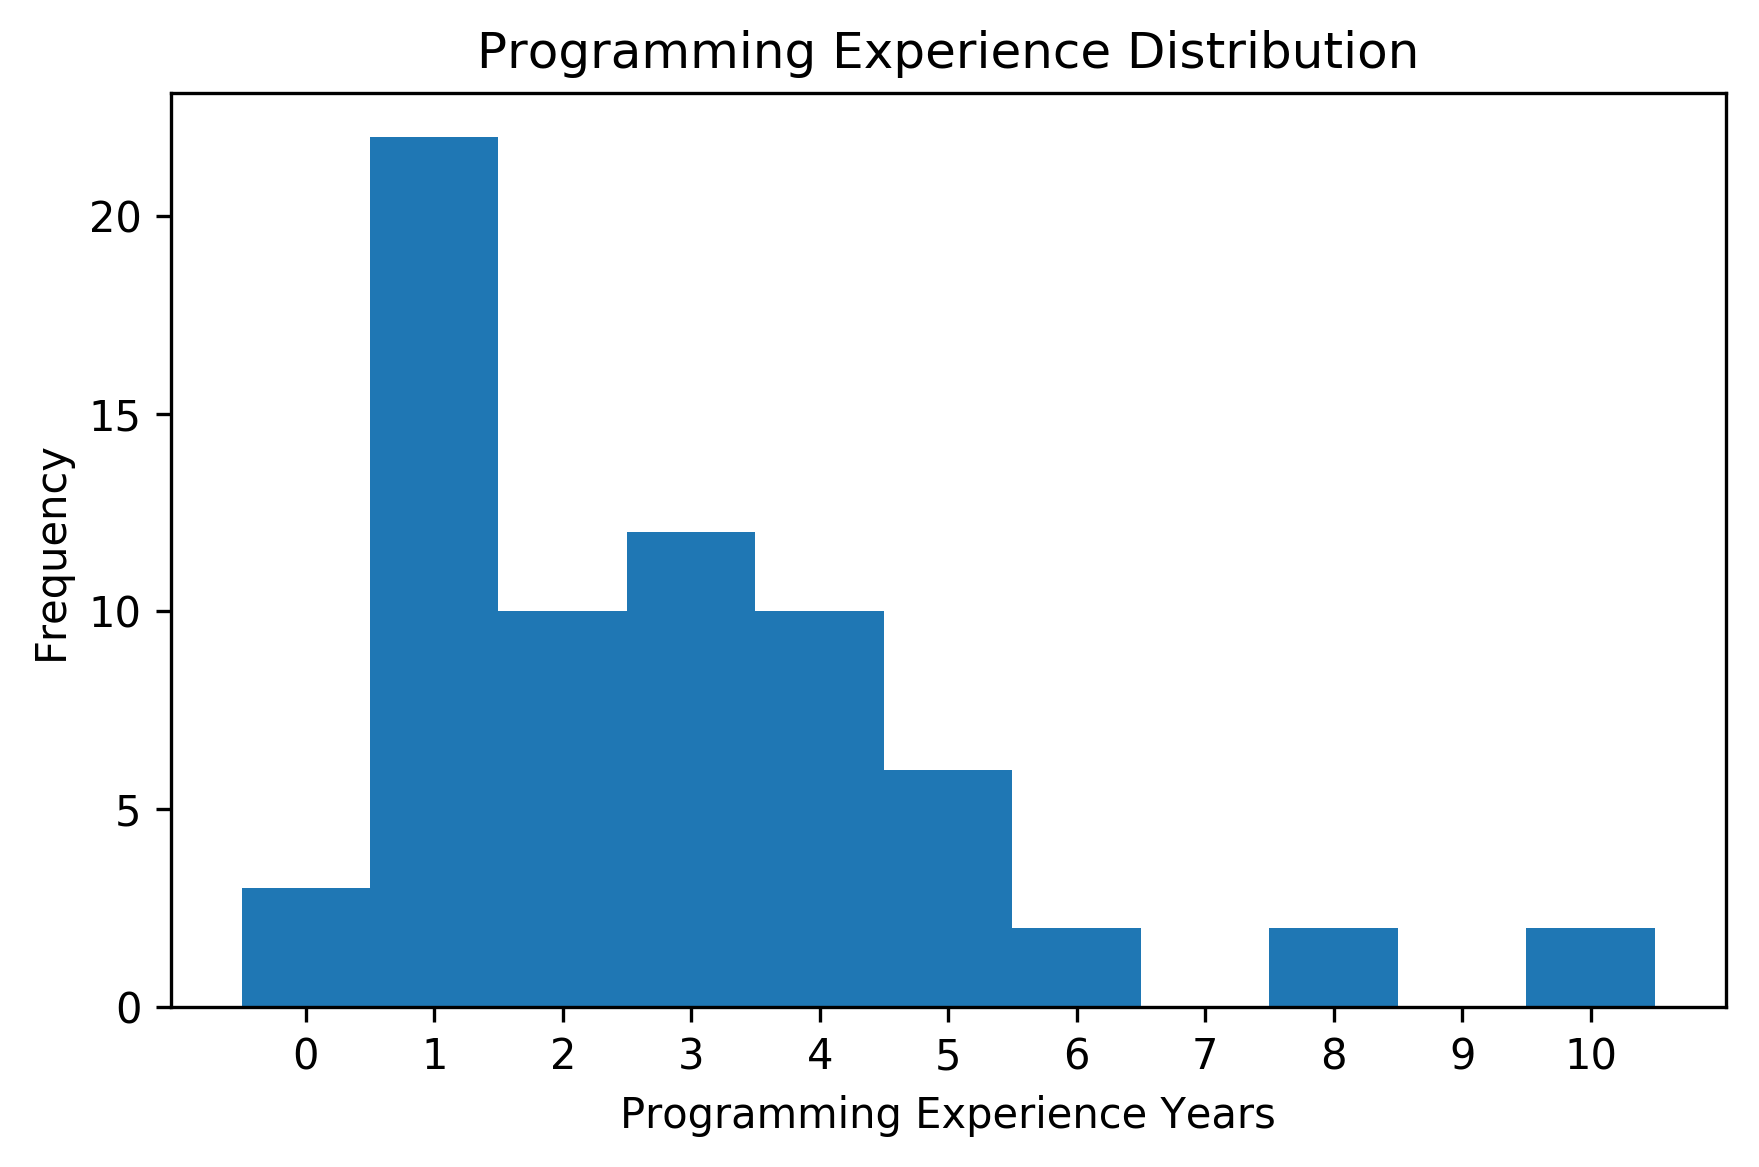
\includegraphics[width=3in]{./figs/programming-experience-distribution.png}
    \caption{Frequency histogram displaying all 69 responses for the programming experience question. A value of 10 means 10 or more years.}
    \label{PROG_EXP}
  \end{figure}
  
  \begin{figure}[ht]
    \centering
    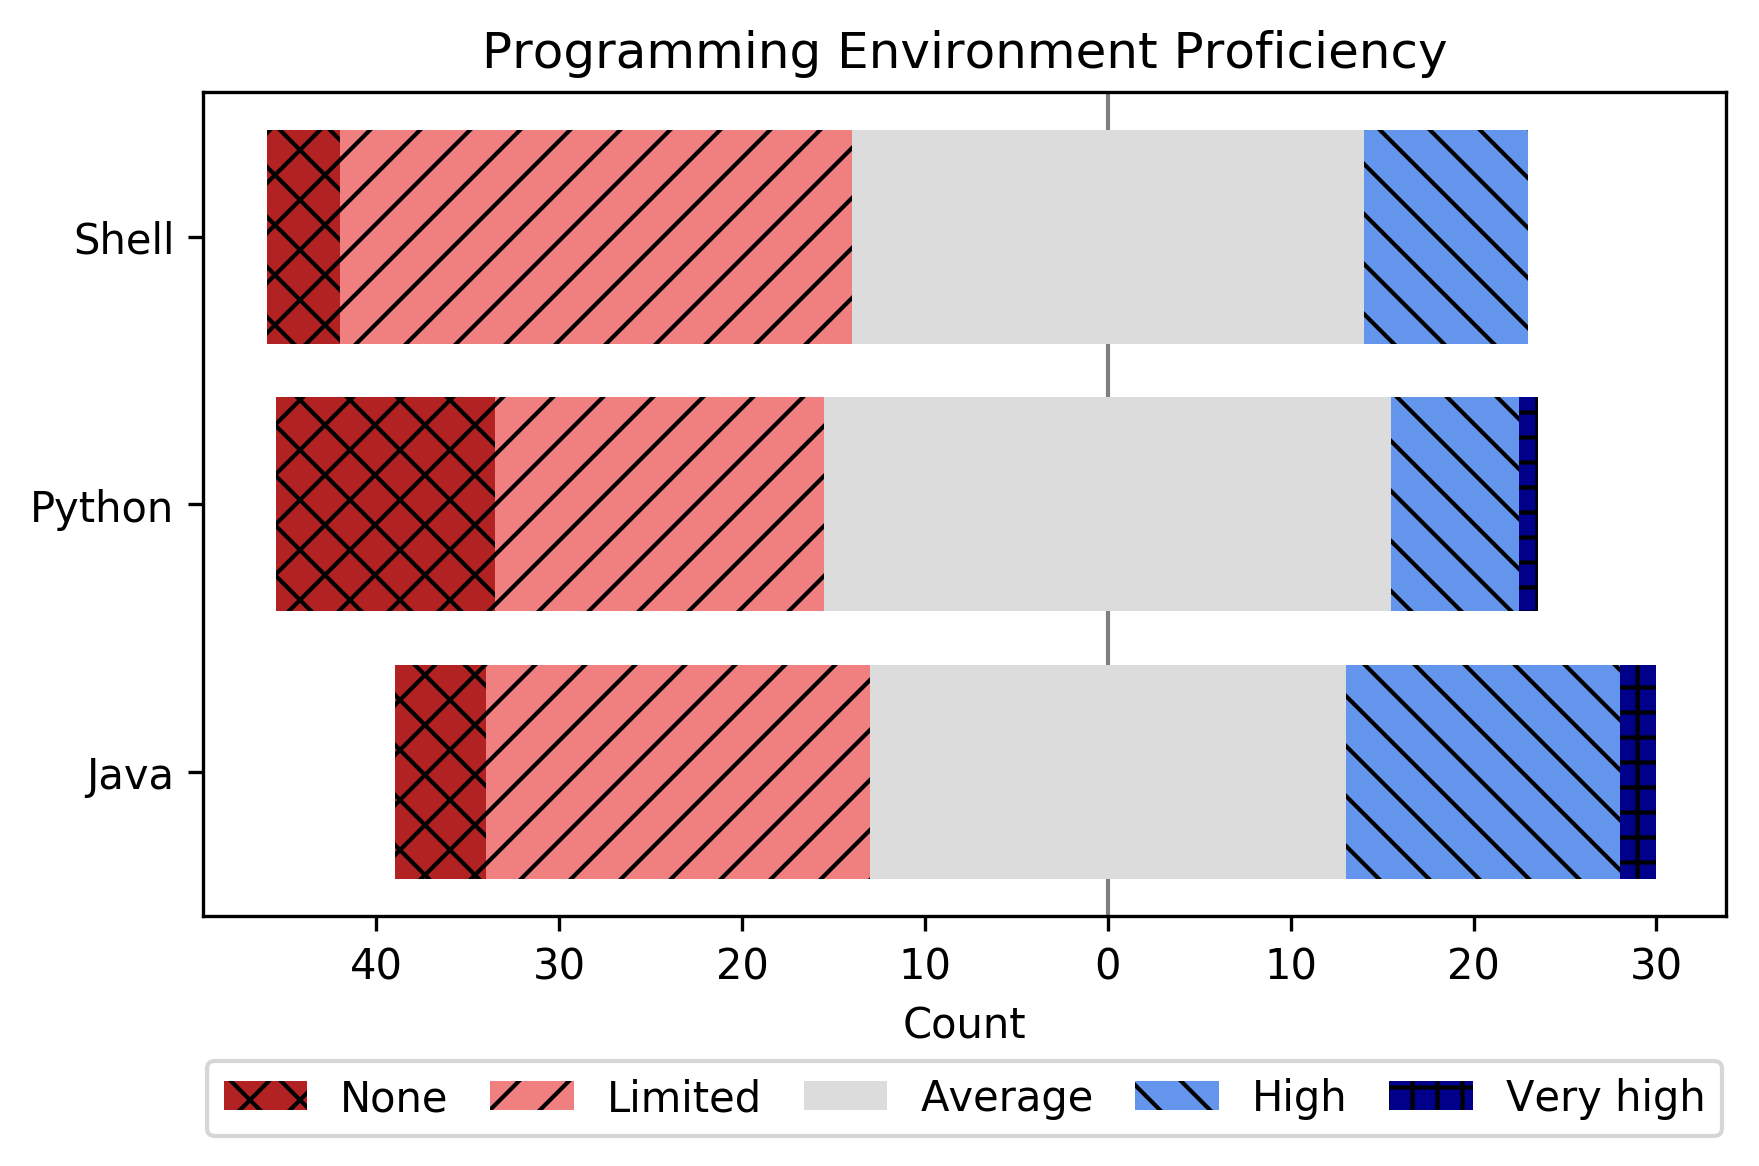
\includegraphics[width=3in]{./figs/programming-environment-proficiency.png}
    \caption{Diverging stacked bar chart \cite{HEIBERGER:DSBC:2014} displaying all 69 Likert scale responses for questions on perceived programming proficiency.}
    \label{PROG_ENV_PROF}
  \end{figure}
  
  Of the 69 participants: 55 were graduate computing students; 7 were Master of Data Science students, who do not necessarily have a computer science background; 6 were final-year undergraduate students; and 1 was a master's student of a different degree.

  Figure~\ref{PROG_EXP} shows that most (78.3\%) participants reported having 1 to 4 years of programming experience. Reflecting the diversity of the student cohort, around half of the participants reported to have limited or no proficiency in shell and Python environments, compared to around a third for Java, as seen in Figure~\ref{PROG_ENV_PROF}. There is a slightly negative correlation between Java and Python proficiency, with a Spearman's rank correlation coefficient of -0.128. The Pearson correlation coefficient was not used because the data is ordinal level, failing the test's ratio level assumption.


\subsection{Preferences and SUS Scores}
\label{PREF_SUS_SCORES}
  
  \begin{figure}[ht]
    \centering
    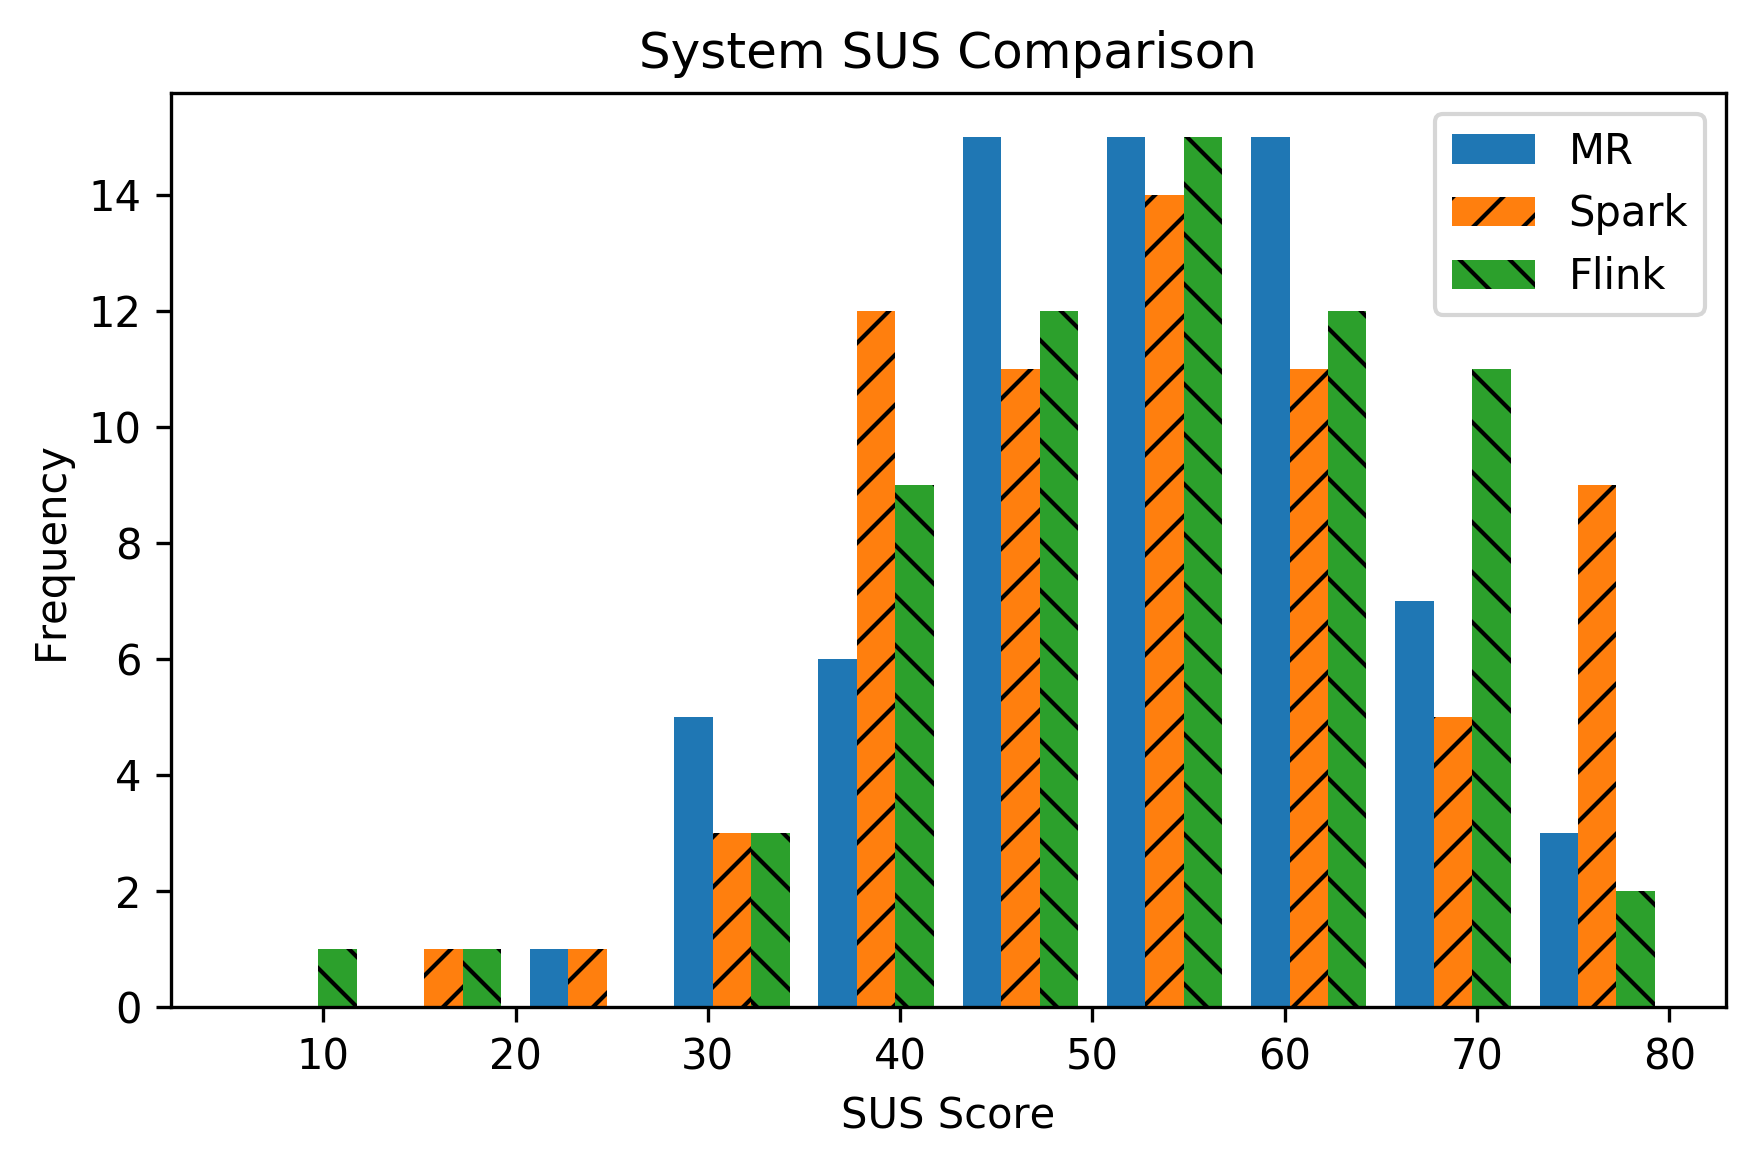
\includegraphics[width=3in]{./figs/system-sus-comparison-histogram.png}
    \caption{Frequency histogram comparing all 69 SUS scores per system (minus 7 individual incomplete responses).}
    \label{SYSTEM_SUS_HIST}
  \end{figure}
  
  \begin{figure}[ht]
    \centering
    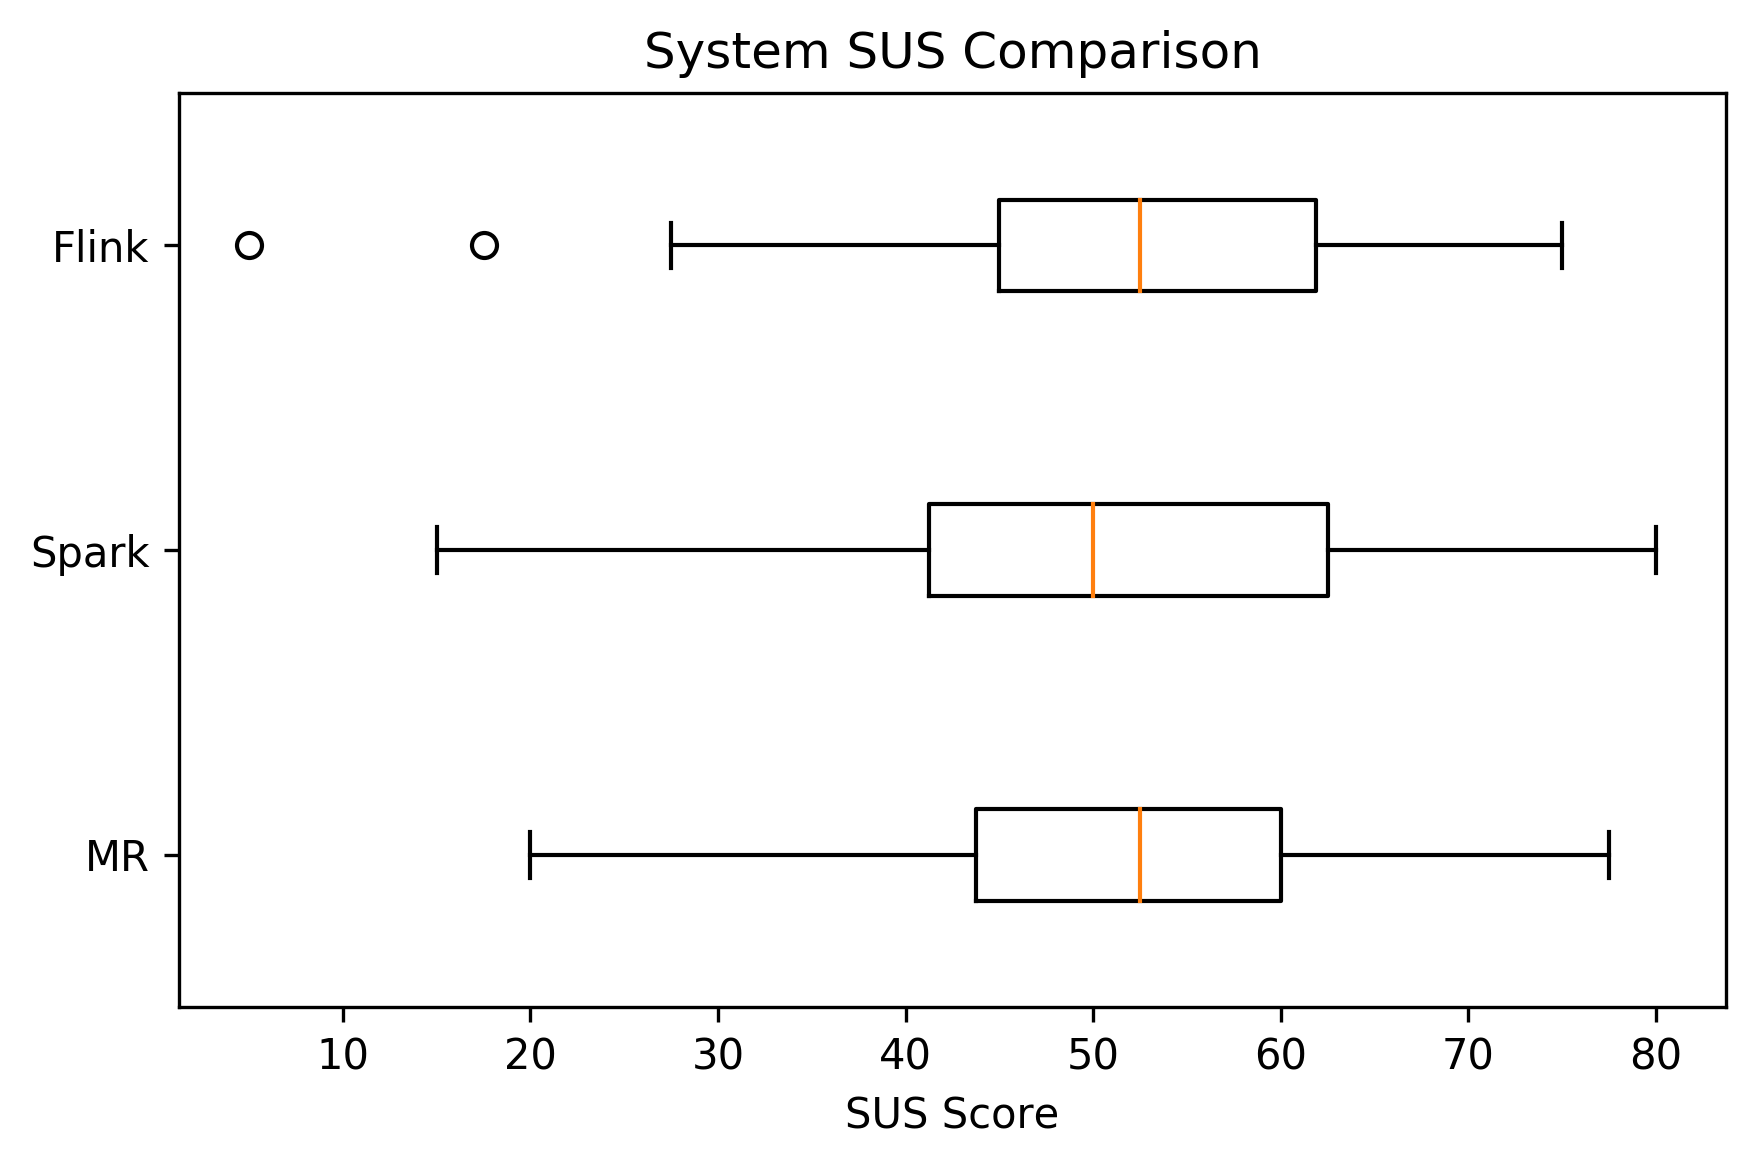
\includegraphics[width=3in]{./figs/system-sus-comparison-boxplot.png}
    \caption{Box and whisker plot comparing all 69 SUS scores per system (minus 7 individual incomplete responses). Whiskers extend to the furthest measurement within 1.5 IQR beyond quartiles. Outliers are circles.}
    \label{SYSTEM_SUS_BOX}
  \end{figure}

  Following the completion of the third survey, participants reported their system preference as: 8 (11.6\%) for Apache Hadoop MapReduce; 29 (42.0\%) for Apache Spark; and 32 (46.4\%) for Apache Flink. This is strong evidence that Spark and Flink were preferred over Hadoop MapReduce.
  
  The difference was similarly pronounced among data science students where 5 of 7 preferred Flink over Spark or MapReduce. However we note that four of those five students did use Flink in assignment~2 before using Spark, which could have an influence, as Section~\ref{ASSIGNMENT_INFLUENCE} will show. Due to the small amount of data in this context there was no applicable significance test. 
  
  The SUS scores reveal little information, with all systems sharing similar distributions and quartiles, as visible in Figures~\ref{SYSTEM_SUS_HIST} and~\ref{SYSTEM_SUS_BOX}. This can be supported by a Friedman test of all participants' three system SUS scores, resulting in a probability ($p$) value of 0.943, which suggests that there is no statistically significant difference between the systems. One-way ANOVA of repeated measures was not used because the data was nonparametric. More specifically, the hypothesis that Apache Flink scores come from a population with a normal distribution can be rejected with a Shapiro-Wilk $p$-value of 0.039 at a significance level of 0.05, and also have outliers as visible in Figure~\ref{SYSTEM_SUS_BOX}. (Hadoop MapReduce and Apache Spark have Shapiro-Wilk $p$-values of 0.767 and 0.352 respectively.)

  While participants have strongly suggested preference of Spark or Flink over MapReduce, there is no clear distinction between the two data processing systems themselves. It also means that the SUS, though a standard measure for system usability, appears to poorly correlate with perceived preferences in this context, as its lack of difference between the systems does not at all reflect the strong separation of MapReduce.


\subsection{Influence of Assignments}
\label{ASSIGNMENT_INFLUENCE}
  
  \begin{figure}[ht]
    \centering
    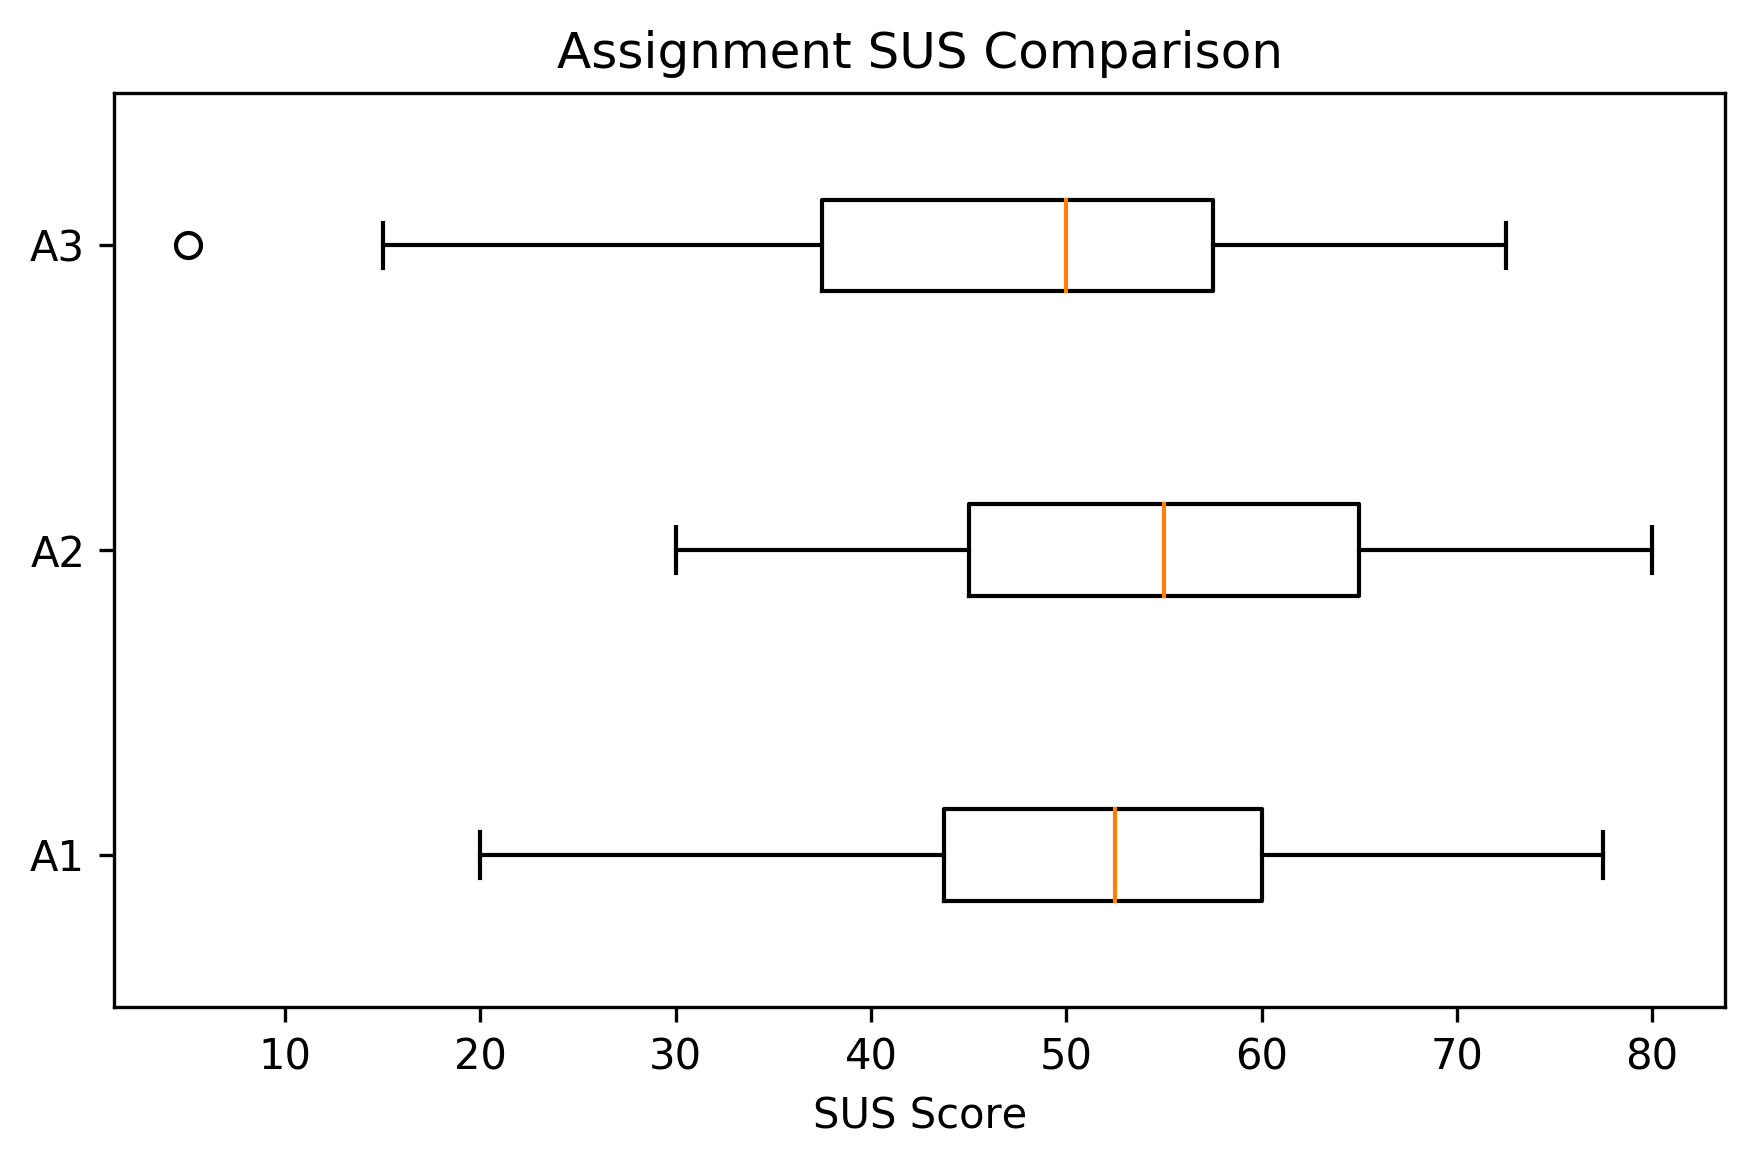
\includegraphics[width=3in]{./figs/assignment-sus-comparison.png}
    \caption{Box and whisker plot comparing all 69 SUS scores per assignment (minus 7 individual incomplete responses). Whiskers extend to the furthest measurement within 1.5 IQR beyond quartiles. Outliers are circles.}
    \label{ASSIGNMENT_SUS}
  \end{figure}
  
  \begin{figure}[ht]
    \centering
    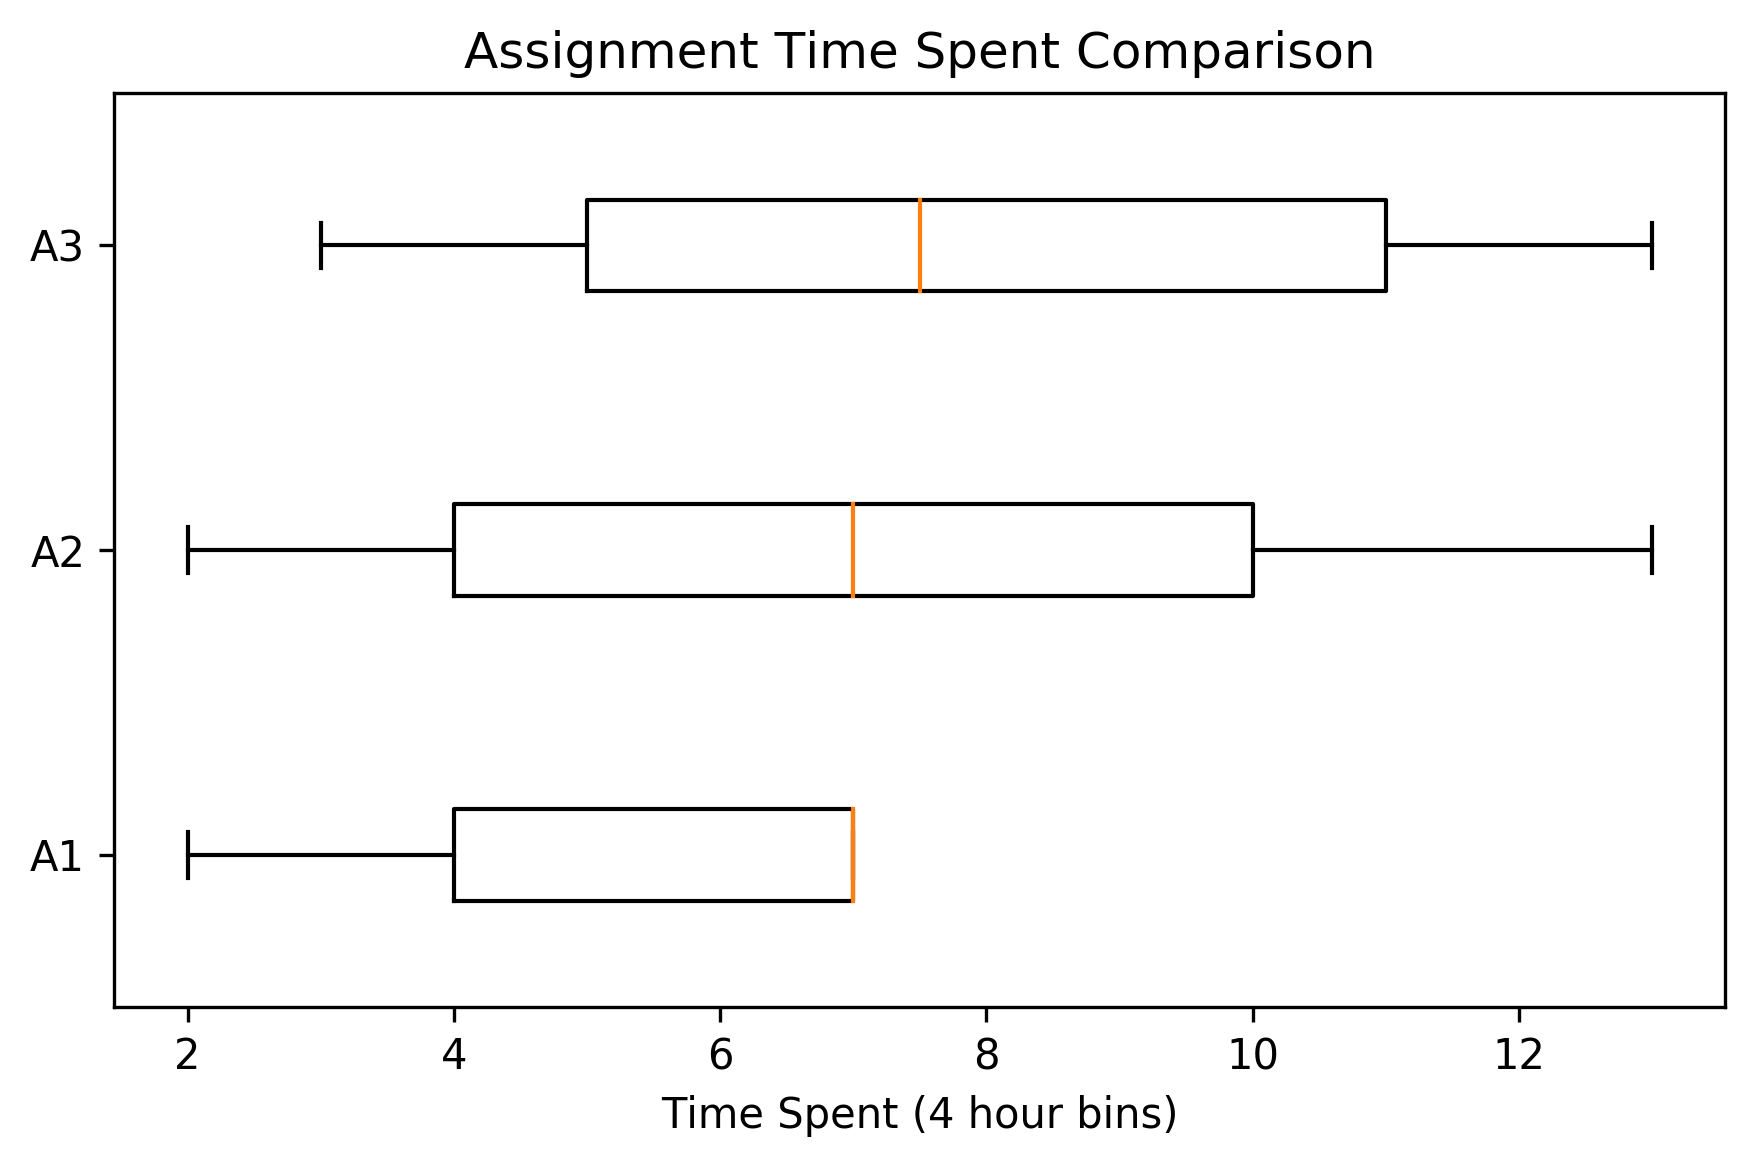
\includegraphics[width=3in]{./figs/assignment-time-comparison-boxplot.png}
    \caption{Box and whisker plot comparing all 69 amounts of time spent per assignment (minus 2 individual incomplete responses). Whiskers extend to the furthest measurement within 1.5 IQR beyond quartiles. A value of 3 means 8-12 hours, and 13 means 48+ hours. Assignment 1 was limited to value 7 or 24+ hours.}
    \label{ASSIGNMENT_TIME_BOX}
  \end{figure}
  
  \begin{figure}[ht]
    \centering
    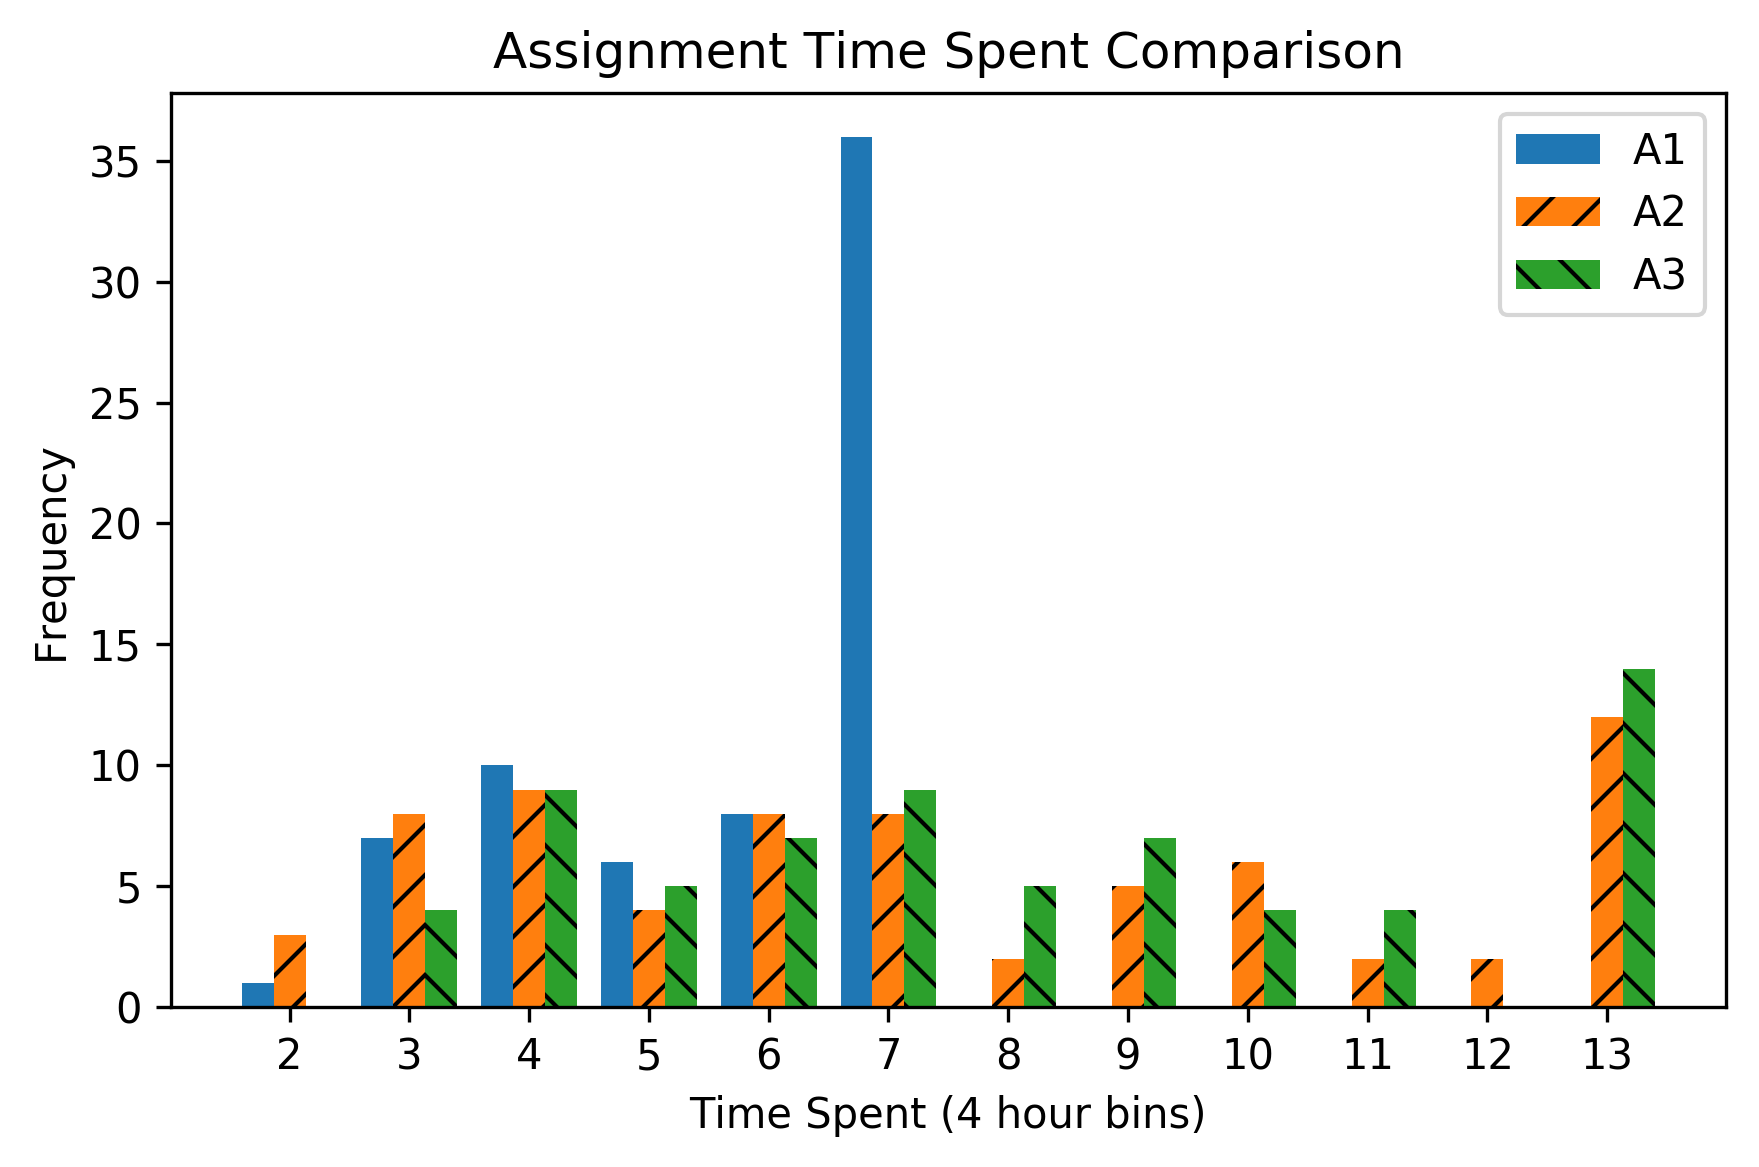
\includegraphics[width=3in]{./figs/assignment-time-comparison-histogram.png}
    \caption{Frequency histogram comparing all 69 amounts of time spent per assignment (minus 2 individual incomplete responses). A value of 3 means 8-12 hours, and 13 means 48+ hours. Assignment 1 was limited to value 7 or 24+ hours.}
    \label{ASSIGNMENT_TIME_HIST}
  \end{figure}

  The usage of a crossed A/B test in assignments~2 and~3 means the SUS scores per assignment differ from the SUS scores per system. The difference in SUS scores is more clearly pronounced per assignment than per system, as visible by comparing Figure~\ref{ASSIGNMENT_SUS} to Figure~\ref{SYSTEM_SUS_BOX}. It appears as though assignment~2 had the highest relative SUS scores, and assignment~3 the lowest. This is supported by a Friedman test of all participants' three assignment SUS scores, resulting in a $p$-value of 0.025, which suggests a statistically significant difference at a significance level of 0.05.
  
  More than half of the participants (39 participants or 56.5\%) preferred the system they used in assignment~2, compared to 22 (31.9\%) for assignment~3 (with the other 8 (11.6\%) preferring Apache Hadoop MapReduce), which is quite a noteworthy difference. However, it is difficult to reason about this difference, as there is no clear distinction as to whether the difference is due to some form of a first-system-used bias or differences in assignment difficulty (as described in Section~\ref{USABILITY_STUDY}). Figure~\ref{ASSIGNMENT_TIME_BOX} shows the time spent working on assignments, which provides a hint as to potential differences in assignment difficulty, wherein assignment~3 appeared to require slightly more time than assignment~2. However, this claim is not supported by a one-sided sign test with plus representing participants who spent more time on assignment~3 than~2, and minus otherwise, resulting in a $p$-value of 0.358. The sign test is used because the data is non-normal and asymmetrical, as clearly visible in Figure~\ref{ASSIGNMENT_TIME_HIST}, ruling out the paired t-test due to it being a parametric test, and the Wilcoxon signed-rank test due to it having high Type I error rates when used with asymmetric data.
  
  While we suspect assignment difficulty and `first-used advantages' could have affected perceived preferences, we have not been able to quantitatively explain the significant difference between assignment SUS scores, nor any link between SUS scores and assignment preferences. With that being said, the crossed A/B test that was used should have helped to reduce any effect of these biases on the systems themselves.


\subsection{Programming Duration versus System}
\label{INF_PROG_DURATION_VS_SYSTEM}
  
  \begin{figure}[ht]
    \centering
    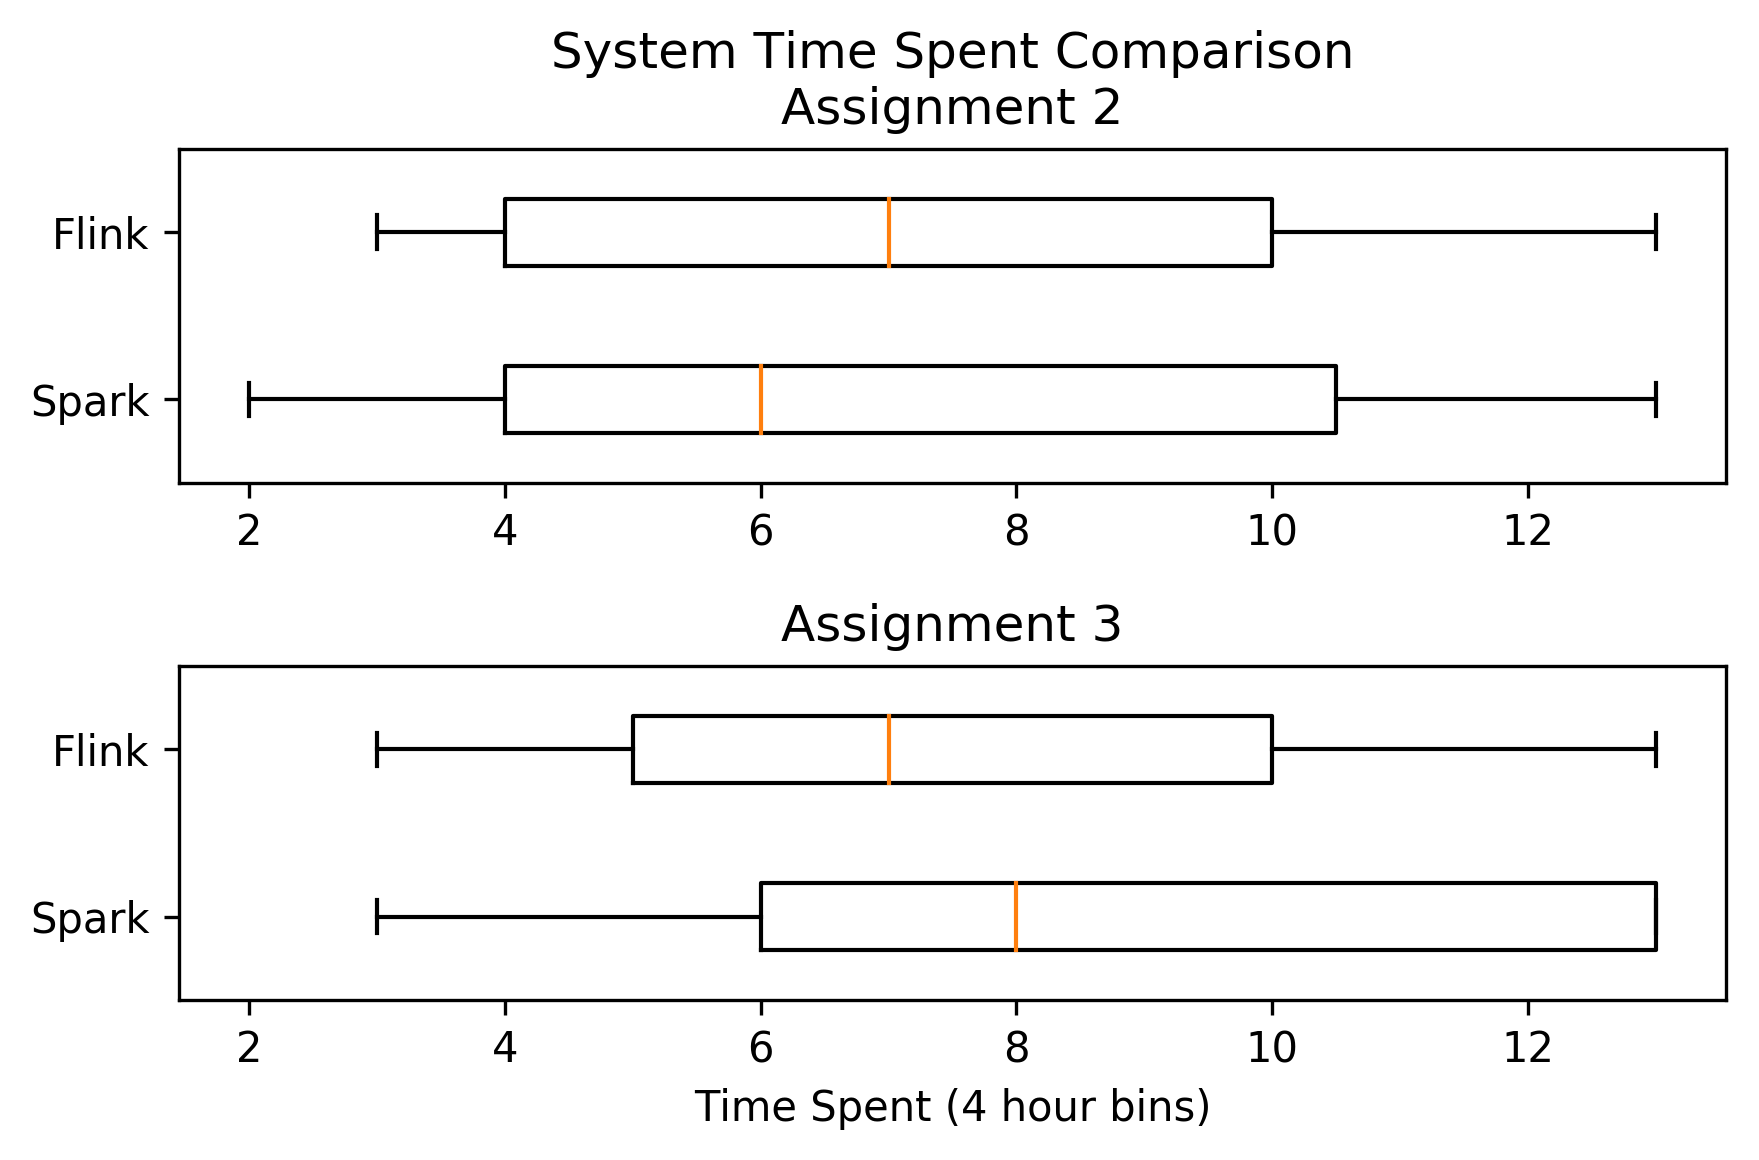
\includegraphics[width=3in]{./figs/assignment-system-time-comparison-boxplot.png}
    \caption{Box and whisker plots for assignments 2 and 3 comparing all 69 amounts of time spent per assignment (minus 1 individual incomplete response). Whiskers extend to the furthest measurement within 1.5 IQR beyond quartiles. A value of 3 means 8-12 hours, and 13 means 48+ hours.}
    \label{ASSIGNMENT_SYSTEM_TIME_BOX}
  \end{figure}
  
  \begin{figure}[ht]
    \centering
    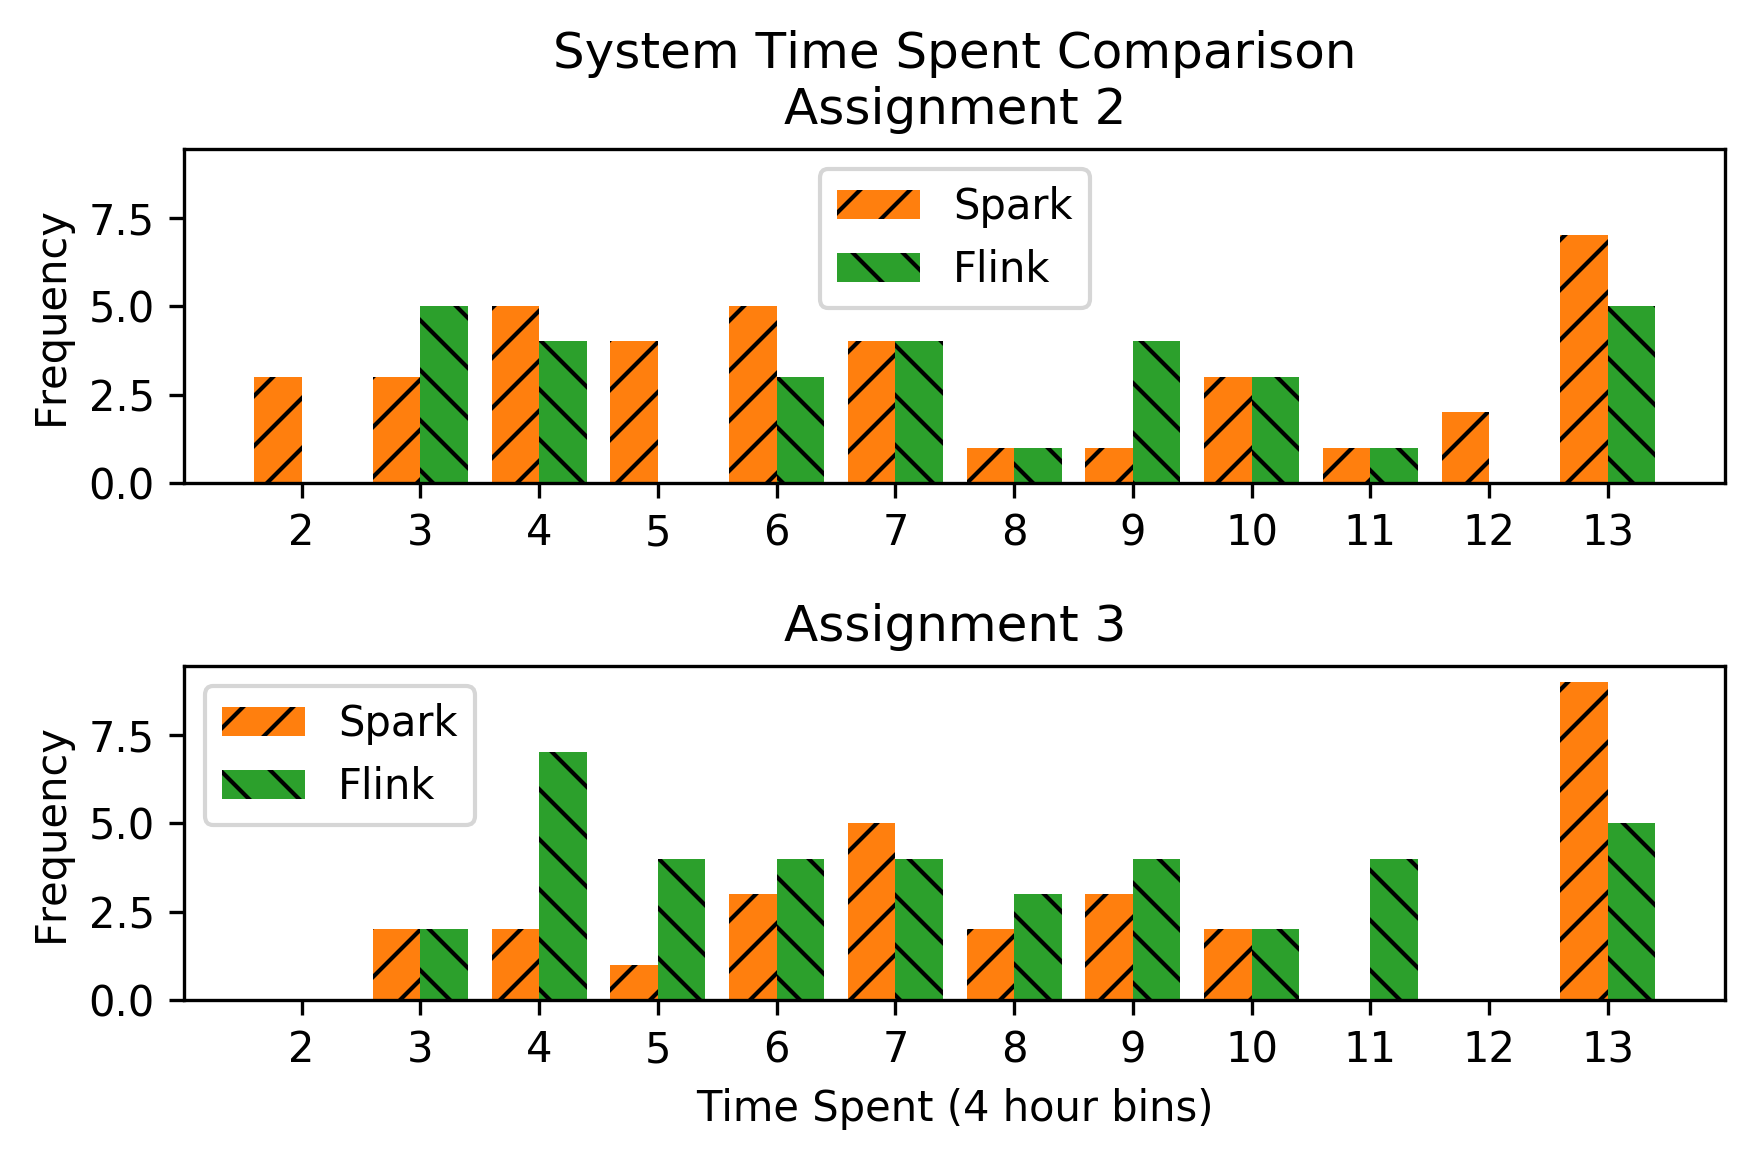
\includegraphics[width=3in]{./figs/assignment-system-time-comparison-histogram.png}
    \caption{Frequency histograms for assignments 2 and 3 comparing all 69 amounts of time spent per system (minus 1 individual incomplete response). A value of 3 means 8-12 hours, and 13 means 48+ hours.}
    \label{ASSIGNMENT_SYSTEM_TIME_HIST}
  \end{figure}
  
  Apache Hadoop MapReduce is not being included in this comparative analysis, as the data we collected for it was unfortunately inappropriate -- described in Subsection~\ref{EXEC_SURVEYS}.

  Apache Spark and Apache Flink shared similar reported development times for assignment~2, but with Flink perhaps showing slightly better results for assignment~3, which you can see in Figure~\ref{ASSIGNMENT_SYSTEM_TIME_BOX}. However, this is not supported by Mood's median tests of the two systems' (independent) time spent data, resulting in $p$-values of 0.661 for assignment~2 and 0.624 for assignment~3, and thus suggesting no statistically significant difference in either. Mood's median test is used because the data is non-normal and differs in distribution, as clearly visible in Figure~\ref{ASSIGNMENT_SYSTEM_TIME_HIST}, ruling out the one-way ANOVA due to it being a parametric test, and the Mann-Whitney U test due to it not testing changes in medians or means (but instead testing changes in distribution) when used with data of differing distributions.

  Spark and Flink do not present a significant difference in the amount of time that was required to complete either of the assignments. This shows that both systems are similarly suitable for completion of data analysis tasks like those in assignments~2 and~3.


\subsection{Influence of Programming Experience}
\label{INF_PROG_EXP}
  
  \begin{figure}[ht]
    \centering
    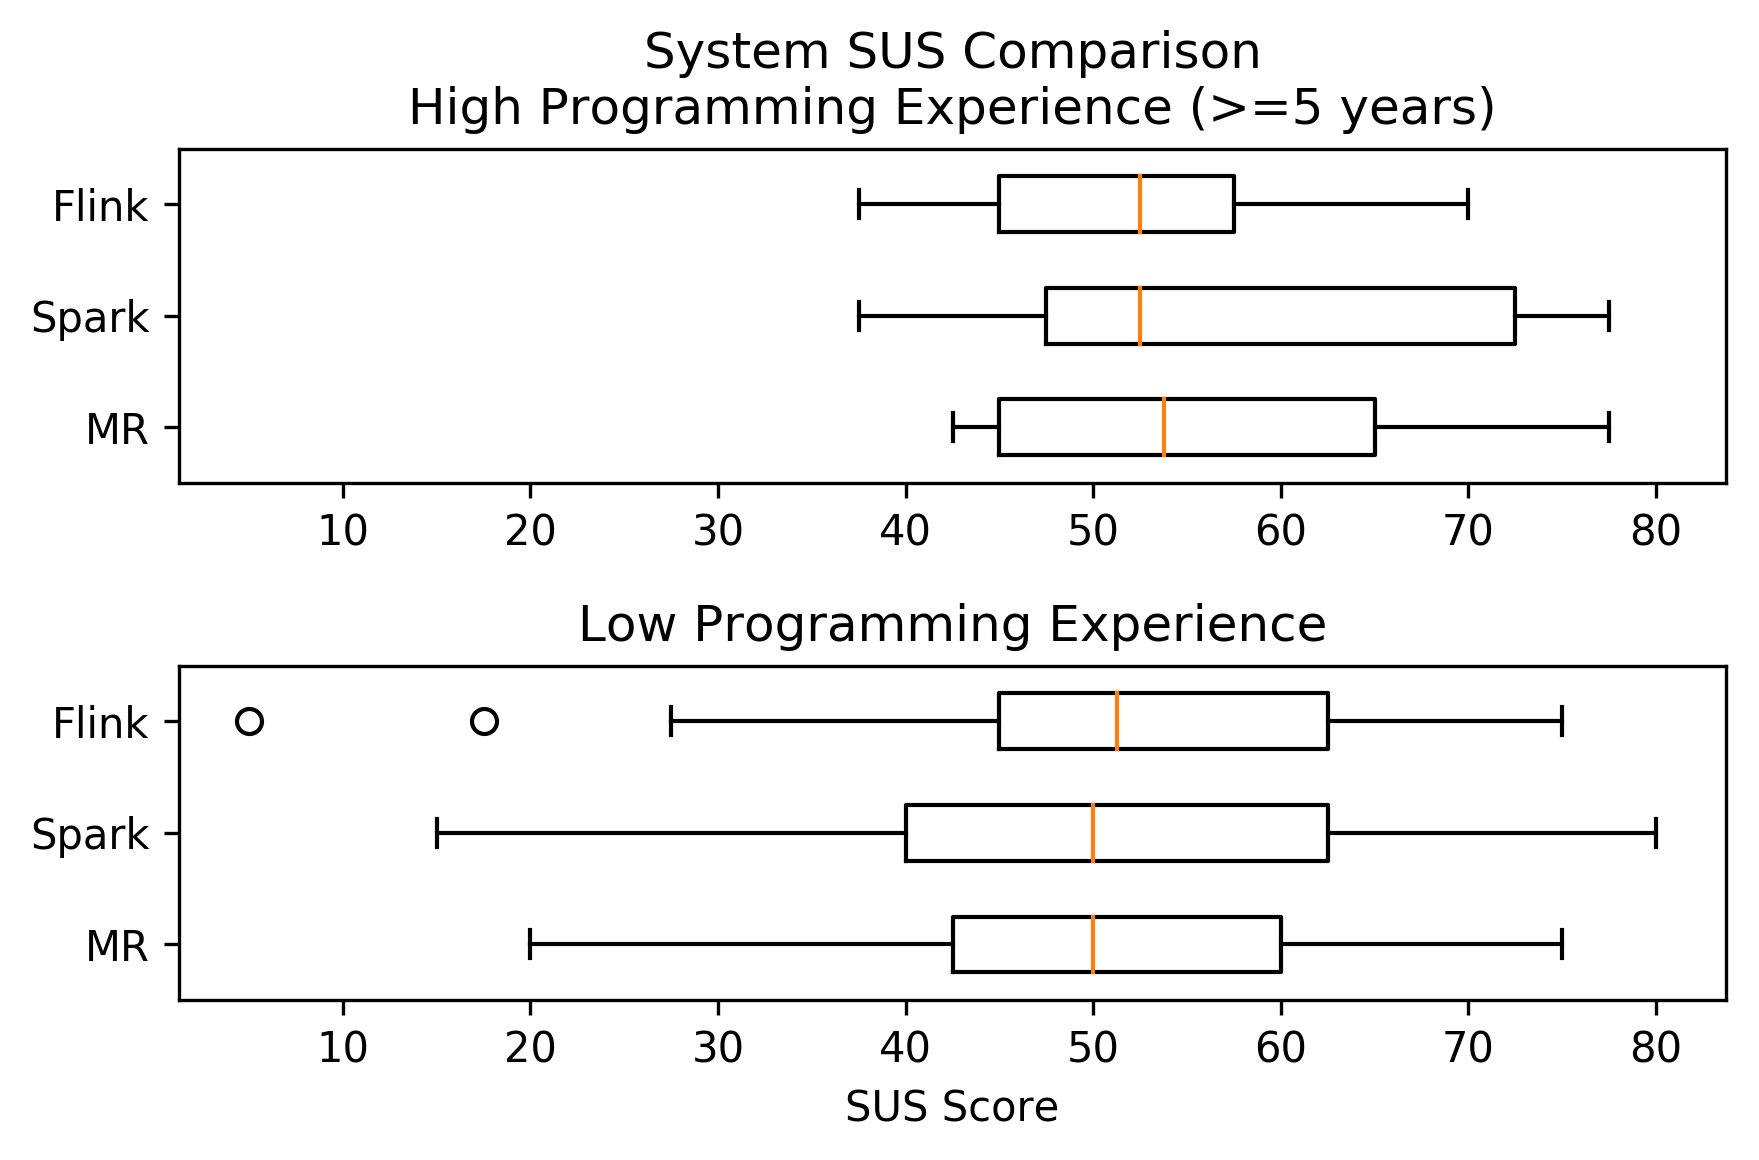
\includegraphics[width=3in]{./figs/exp-system-sus-comparison.png}
    \caption{Box and whisker plots for high (\textgreater=5 years) and low programming experience participants comparing all 69 SUS scores per system (minus 7 individual incomplete responses). Whiskers extend to the furthest measurement within 1.5 IQR beyond quartiles. Outliers are circles.}
    \label{EXP_SYSTEM_SUS}
  \end{figure}
  
  \begin{figure}[ht]
    \centering
    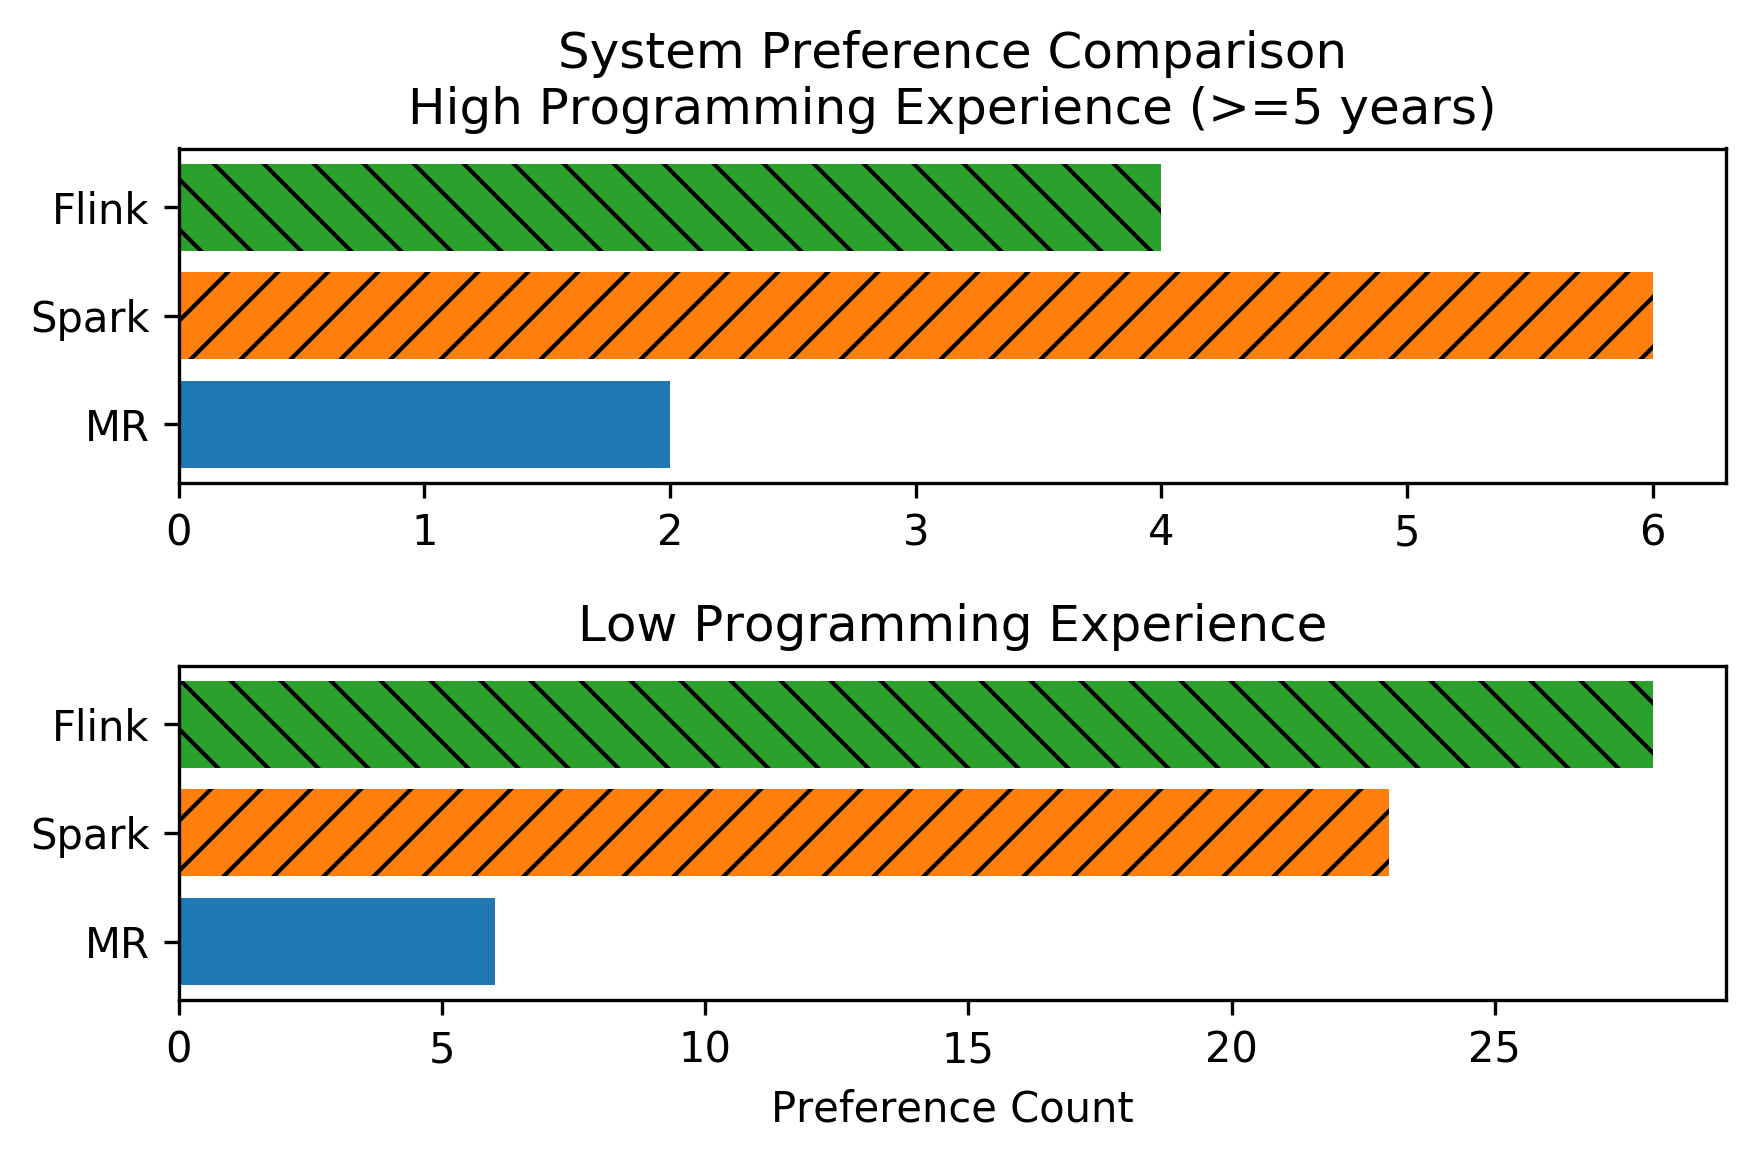
\includegraphics[width=3in]{./figs/exp-system-preference-comparison.png}
    \caption{Bar charts for high (\textgreater=5 years) and low programming experience participants comparing reported system preference counts upon completion of assignment~3. There are 69 preferences measured in total. Charts have differing Preference Count scales.}
    \label{EXP_SYSTEM_PREF}
  \end{figure}

  As previously mentioned, Figure~\ref{PROG_EXP} shows that most (78.3\%) participants reported having 1 to 4 years of programming experience. In this subsection we will consider the 12 (17.4\%) participants who reported having more than 4 years experience as being of relatively `high experience'. Their experience is distributed as so: 6 with 5 years experience, and 2 with each of 6, 8 and 10+ years experience. Is there any difference in the reported preferences or SUS scores for high experience participants compared to the majority?
  
  A comparison between the two groups' system SUS scores is shown in Figure~\ref{EXP_SYSTEM_SUS}, which does not tell much of any preference or skew. The ranges of all three systems are more dense and perhaps slightly higher overall in the high experience group, and also particularly lacking the long tail towards lower scores. However, it is difficult to indicate that it is not due to coincidence. These observations still apply, perhaps with a slight reduction in density, when moving the threshold from 5 years to 3 years and thus placing 34 (49.3\%) participants in the high experience tier.
  
  A comparison between the two groups' reported preferences is shown in Figure~\ref{EXP_SYSTEM_PREF}, which also does not tell much of any preference or skew. Hadoop MapReduce remains behind the dataflow engines, but it is difficult to reason much further. For instance, the difference in Apache Flink and Apache Spark looks quite pronounced, with Flink appearing to be less preferred to Spark in comparison to the low experience group. However, in actual fact it is only a difference of two individual preferences, which is difficult to claim as being anything other than coincidence. When moving the threshold from 5 years to 3 years and thus placing 34 (49.3\%) participants in the high experience tier, the two charts end up look nearly identical, also with very similar Preference Count scales.
  
  It was good to have collected the programming experience data as part of the survey, especially with full participation in that regard, having provided information regarding the background of participants and the diversity present in the study. However, this information did not turn out to be indicative of any pattern in reported preferences or system SUS scores.


\subsection{Influence of Programming Language}
\label{LANGUAGE_INFLUENCE}

  In the analysis thus far, participants' usage of Python or Java for each system or assignment has not been taken into account. However, it is mentioned in Section~\ref{EXECUTION} that learning materials, or more specifically tutorial exercises and sample assignment solutions, were not successfully created for Apache Flink; that students were recommended not to use Python for Flink; and that this recommendation was followed by all students. Unfortunately, this presents an inconsistency in the experiment which could bias some of the findings. This subsection will explore said biases by comparing the previous analyses with a repetition of them that excluded all Python user data.
  
  Of the 69 participants whose data was used in the above analyses, 32 (46.4\%) had used Python for either or both of assignment~1 (Hadoop MapReduce) or the assignment in which they used Apache Spark. Excluding this data leaves 37 records to work with. Furthermore, the crossed A/B test that was employed did not take programming language usage into account, and thus the Python records removed could have further produced skew in that regard. With 69 records the Spark vs. Flink usage split for assignment~2 (and conversely for assignment~3) is 39 vs. 30 (56.5\% vs. 43.5\%) respectively, skewed due to students' requests to switch to Apache Spark as described in Section~\ref{EXECUTION}, whereas with 37 records it is 23 vs. 14 (62.2\% vs. 37.8\%) respectively. Flink is 9 users behind Spark (for assignment~2) in both cases, however this difference is more pronounced as a percentage in the latter case.
  
  Of the subsections that were analysed earlier, noteworthy differences were only apparent in relation to the background of participants, and their reported system preferences.
  
\subsubsection{Background of Participants}
  
  \begin{figure}[ht]
    \centering
    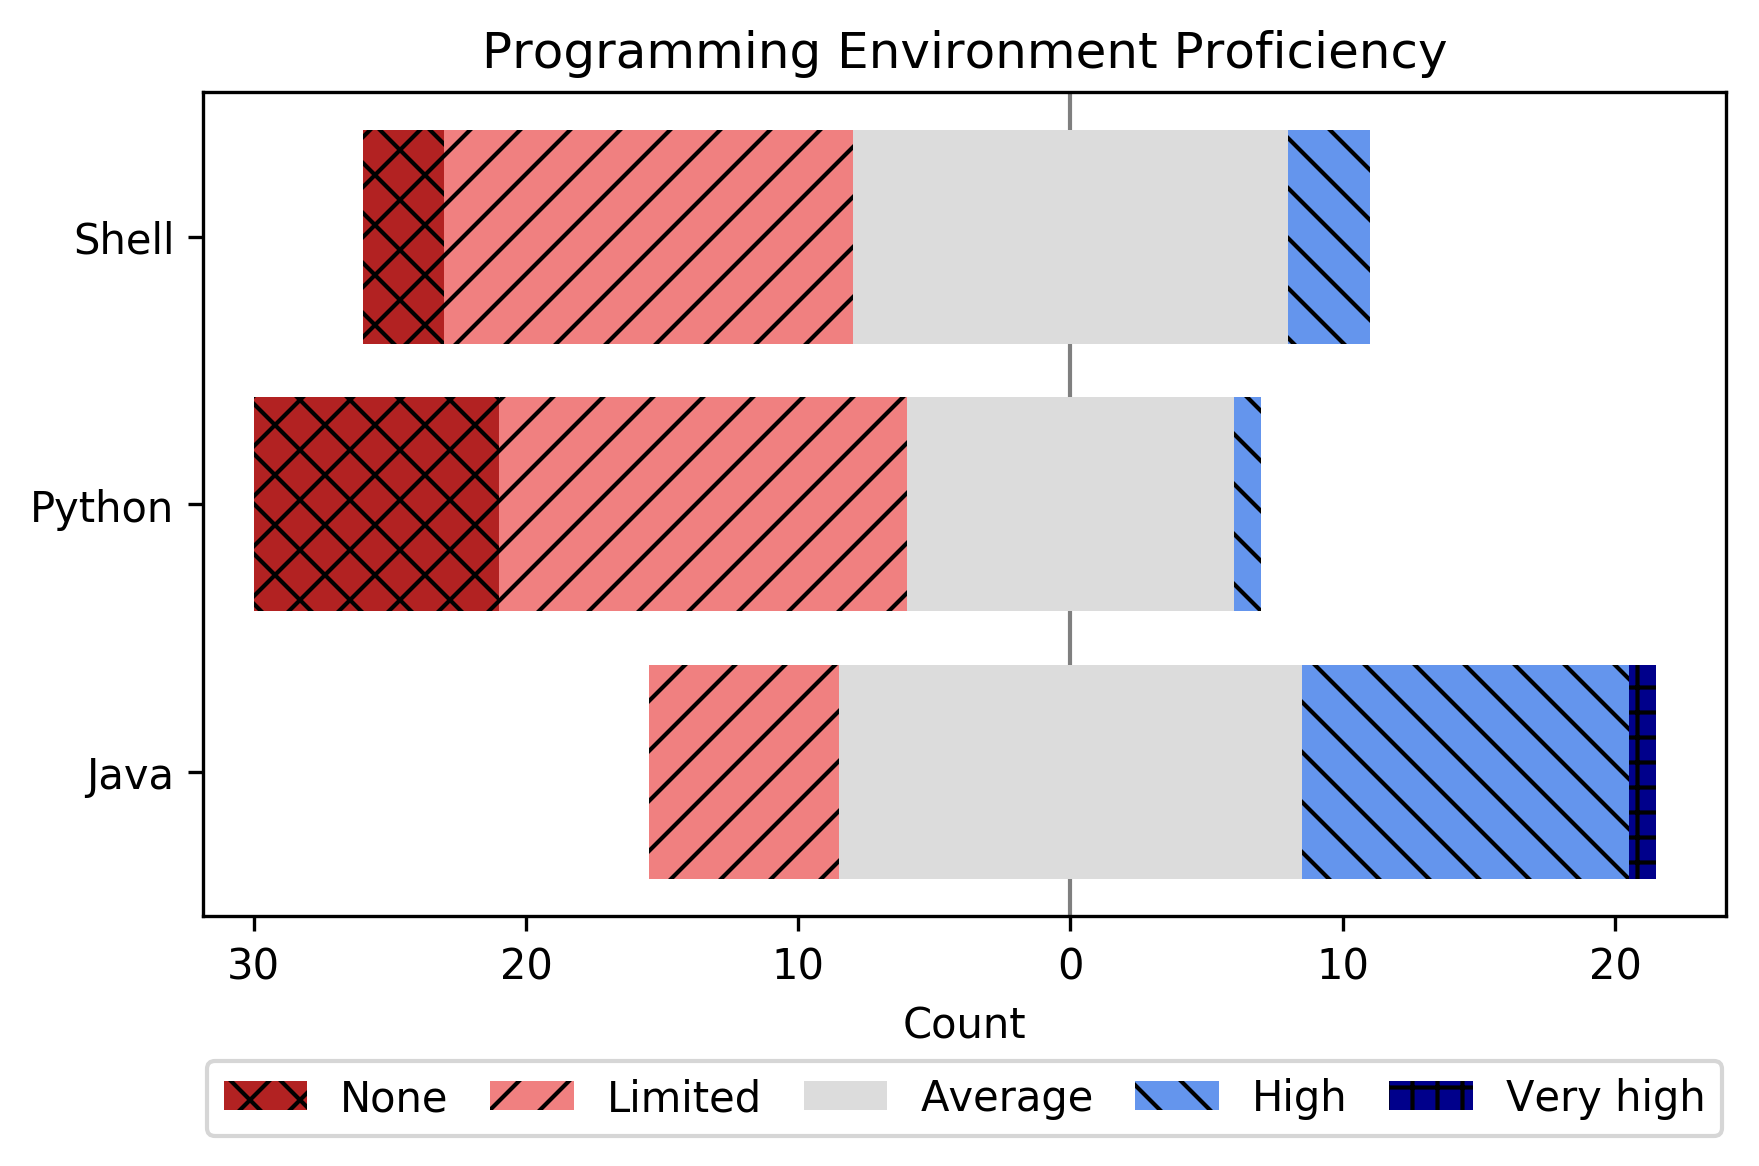
\includegraphics[width=3in]{./figs/nopy-programming-environment-proficiency.png}
    \caption{Diverging stacked bar chart \cite{HEIBERGER:DSBC:2014} displaying all 37 (Python user data excluded) Likert scale responses for questions on perceived programming proficiency.}
    \label{NOPY_PROG_ENV_PROF}
  \end{figure}

  Of the 37 participants: 33 were graduate computing students; 1 (compared to 7) was a Master of Data Science student; 2 were final-year undergraduate students; and 1 was a master's student of a different degree. Furthermore, Figure~\ref{NOPY_PROG_ENV_PROF} (compared to Figure~\ref{PROG_ENV_PROF}) shows the dominance of Java among the cohort, also with substantially more participants reporting having limited or no Python proficiency than average or higher.
  
  This apparent reduction in diversity may be due to individuals in this cohort having been more likely to have come from a computer science background, where compiled and object-oriented programming languages would be of a larger focus than scripting languages -- which is what we observe Python to be commonly taught as, despite it also being object-oriented. Unfortunately, this representation may not effectively capture the experiences of interdisciplinary users, as has been one of our intentions in conducting this study.


\subsubsection{Preferences}

  Following completion of the third survey, participants reported their system preference as: 4 (10.8\%) for Hadoop MapReduce; 12 (32.4\%) for Apache Spark; and 21 (56.8\%) for Apache Flink. While this result is similar to the full (Python included) data set in how MapReduce is behind in comparison to the dataflow engines, it differs from having Spark and Flink on a very close footing to instead placing Flink quite noticeably ahead as the participants' preferred system.
  
  This difference seems to make sense considering that Python users likely felt inconvenienced by the inability to use Python for Flink in comparison to Spark or MapReduce, thus reducing Flink's popularity among the full cohort. With Python users excluded from analysis, it has now become apparent that Flink is preferred over Spark among Java users.
  
  Unfortunately, as described in Section~\ref{EXEC_SURVEYS}, there is little information available from participants to justify these reported preferences, and so we can make no conclusion as to why Java users may have preferred Flink over Spark, especially considering the similarities in their usage as described in Section~\ref{SYSTEMS}. The key difference in usage that we could think of was in Flink's availability of \texttt{IterativeDataSet}, which could have been used in solving both assignments~2 and~3.
  
  With the full data set it was apparent that participants tended to prefer the system they used for assignment~2 more than assignment~3, as described in Section~\ref{ASSIGNMENT_INFLUENCE}. With Python data excluded, this changes to having 17 (45.9\%) participants preferring the system used for assignment~2 compared to 16 (43.2\%) for assignment~3 (with the other 4 (10.8\%) preferring MapReduce). It makes sense that assignment~3 gained preference considering the skewed crossed A/B test distribution, where more participants used Flink for assignment~3, in combination with participants' higher preference of Flink. This means that although reported preferences put assignments~2 and~3 on similar proportions, it remains likely that assignment~3 was somehow disadvantaged.


\subsection{Individual SUS Statements}
\label{SUS_INDIV}
  
  \begin{figure}[ht]
    \centering
    \makebox[\textwidth][c]{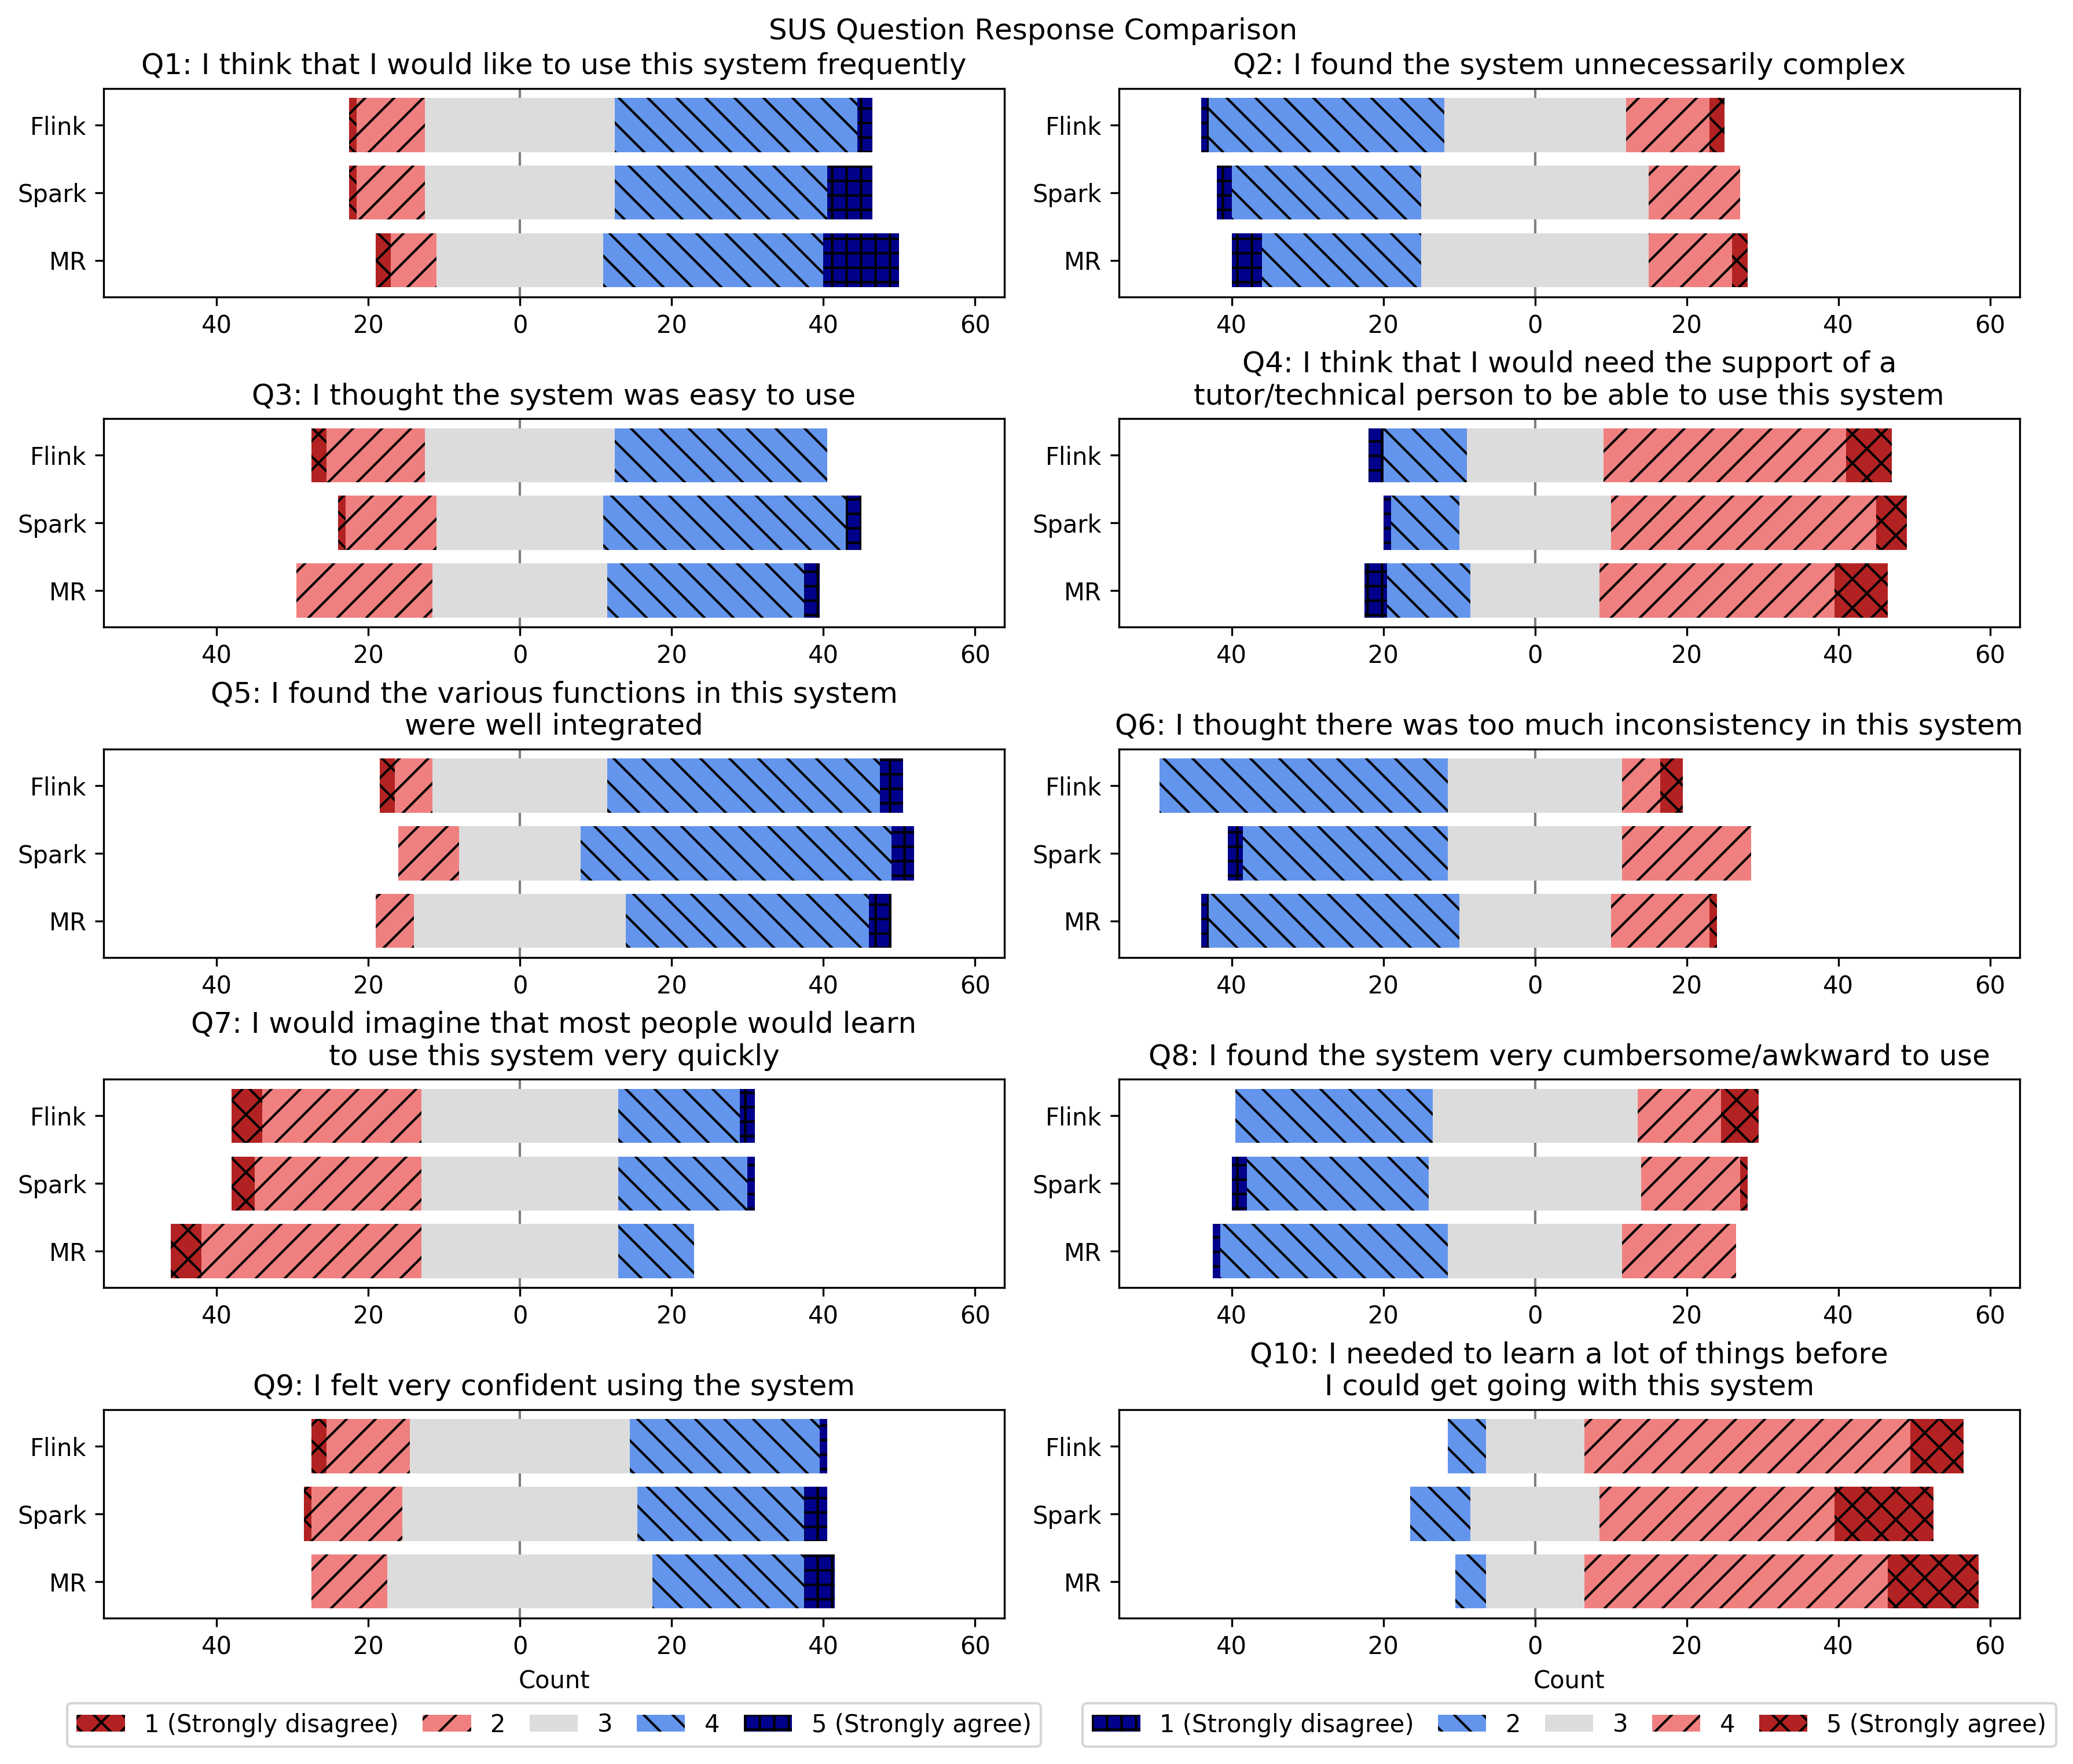
\includegraphics[width=6in]{./figs/sus-questions.png}}
    \caption{Diverging stacked bar charts \cite{HEIBERGER:DSBC:2014} displaying all 69 Likert scale responses for each SUS statement, however minus some missing individual responses. The five odd numbered statements on the left are `positively natured', such as ``Q3: I thought the system was easy to use'' -- agreeing with this statement is \emph{good} in terms of the system's usability. The five even numbered statements on the right are `negatively natured', such as ``Q2: I found the system unnecessarily complex'' -- agreeing with this statement is \emph{bad} in terms of the system's usability. To display this effectively, the legends on the left and right have their colours inverted -- blue is used to highlight good responses (regardless of a statements' positive/negative nature) and red for bad responses.}
    \label{SUS_QS}
  \end{figure}
  
  This subsection will discuss Figure~\ref{SUS_QS}, which displays all participants' responses to all ten SUS statements. The figure has been organised in a particular way considering the nature of the SUS. Its caption describes the intended interpretation.
  
  The first takeaway is that, for all ten questions, there is little difference in response distribution between the three systems. This explains why the SUS scores were very similar, as discussed in Section~\ref{PREF_SUS_SCORES}. It shows that in terms of usability as examined by the System Usability Scale, these three systems apparently share the same strengths and weaknesses, which is unintuitive considering that Apache Spark and Flink feature much higher level APIs.
  
  Furthermore, most questions had a good response as either a slight or strong majority -- a good sign for the usability of these systems. There are three exceptions: ``Q4: I think that I would need the support of a tutor/technical person to be able to use this system'', which most participants agreed with; ``Q7: I would imagine that most people would learn to use this system very quickly'', which a slight majority of participants disagreed with; and ``Q10: I needed to learn a lot of things before I could get going with this system'', which participants overwhelmingly agreed or strongly agreed with.
  
  These three questions with bad responses cover the topics of learning and support, and are the only questions in the set of ten concerning them. The other seven questions with good responses covered topics such as ease of use and system design and complexity. Is it normal that participants perceived the systems to be well designed, non-complex and usable, and yet hard to learn and in need of support to be used? One interpretation of this result is that participants felt that the systems were to be complex by design, considering their function as distributed computing engines, and in that context perceived them to be usable and such.
  
  However, the steep learning curve still needed to be addressed for them to use the system. We believe this is indicative of a prominent barrier to adoption of data science systems -- although they effectively abstract various distributed computing and dataflow challenges away, without simplifying the process of learning to use and overcoming difficulties with these systems, users with non-computing backgrounds will have significant trouble adopting them. From our experience and from the feedback of participants, we found the key areas for improvement to be first-party documentation and the process of debugging programs.


\subsection{Free-text Feedback and Other Impressions}
  
  Considering the participants' free-text feedback, and the experiences of instructors throughout execution of the study and teaching of its materials, we are able to highlight several areas of potential future improvement of the evaluated systems:
  
  \begin{itemize}
    \item Debugging in MapReduce was particularly difficult.
    \item MapReduce code tended to be overly verbose.
    \item Flink development environment setup was troublesome.
    \item Python support in Flink 1.2 felt immature.
    \item Spark and Flink felt quite similar to work with.
    \item Spark and Flink documentation covered basic usage quite well, but was limited for non-standard operations. Consequently, both Spark and Flink involved significant trial and error.
    \item Spark community support was good, but first-party documentation was lacking. Flink was described inversely.
  \end{itemize}
  
  We note that these points represent anecdotal observations only, but believe they are a good indicator of the general struggles faced by new users of these systems. Considering them, we would recommend that developers of these newer dataflow engines work to excel in regards to the on-boarding experience, the process of debugging, and the documentation of these systems -- especially for non-standard operations, perhaps by providing a very wide range of examples as opposed to focusing on canonical ones. Work in these suggested areas would complement the already greatly improved usability that  these systems provide, giving new users a streamlined experience of adoption, which is especially beneficial for individuals from non-distributed computing backgrounds.